In this chapter the implementation details are introduced and the evaluation of the AppElastic algorithm with prediction accuracy is presented. This chapter start with presentation of simulator called ElasticSim. Then details about the implementation of prediction algorithm presented. In Section~\ref{sec:AppElastic Algorithm Implementation}, details about the implementation of AppElastic algorithm is explained with few code snippets. In the later sections of this chapter accuracy of the prediction is discussed and the effectiveness of the AppElastic algorithm is presented.

\section{ElasticSim}
\label{section:ElasticSim}
Design of the ElasticSim was introduced in previous chapter and its three layers: Configuration, Prediction and Simulation Core layers, were presented. The implementation details of ElasticSim is discussed in this section.

\subsubsection{Technology Selection}
\label{subs:Technology Selection}
ElasticSim is composited of various technologies. The configuration layer and simulation core is implemented in Java\footnote{http://java.net/}. Where as the prediction layer is implemented in R scripting language~\cite{rstat}. These two layer are interconnect with a Bash script\footnote{https://www.gnu.org/software/bash/}.

\subsubsection{ElasticSim Operation}
\label{subs:ElasticSim Operation}
ElasticSim at a high level provides four different operations. These operations are provided at the start of the simulator. The start screen of the simulator is as shown in the Figure~\ref{figure:simwelcome}. These options serves four different functionality, this is as described below:

\begin{enumerate}
  \item First option consist of R scripts which implements the prediction functionality. The prediction script reads the workload trace file, split the input into two half, for testing and training, and runs ARIMA forecast model.
  \item Second option runs the AppElastic algorithm on historical workload traces, so that the simulation users can decide on number of reserved instances to choose for reservation.
  \item Third options runs the AppElastic algorithm on a given workload trace and considers different instance types. Here the user specify number of reserved instances to use for this simulation run.
  \item Fourth options runs the AppElastic algorithm to generate the simulation logs so that a newly built scaling algorithm can be tested easily.
\end{enumerate}

\begin{figure}[h]
  \begin{center}
    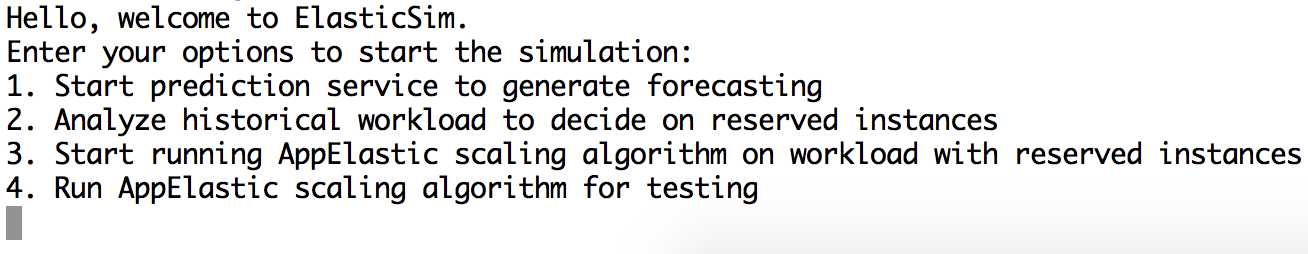
\includegraphics[scale=0.6]{simwelcome.png}
    \caption{ElasticSim}
    \label{figure:simwelcome}
  \end{center}
\end{figure}

\subsubsection{Input to ElasticSim}
\label{subs:Input to ElasticSim}
Inputs to ElasticSim is provided through a simple configuration interface. This simulator configuration file is as show in the Figure~\ref{figure:simconfig}. ElasticSim uses these configuration values for providing input for the algorithm. These configurations can be grouped into five types: VM configuration, AppElastic configuration, Cloud service provider related configuration, Workload trace configuration, Output log configuration. These types can be explained as follows:

\begin{itemize}
  \item VM configuration include VM startup and shutdown time. These time is configured through the variable VM\_START\_TIME and VM\_SHUTDOWN\_TIME respectively.
  \item Since AppElastic is a threshold based algorithm. Threshold can be easily configured by assigning values to NUMBER\_OF\_USERS\_PER\_INSTANCES variable. Lookahead period for AppElastic can be configured through LOOKAHEAD\_SCALEUP and LOOKAHEAD\_SCALEDOWN variables.
  \item Cloud service provider related configuration includes instance purchasing, billing period. To configure different instance pricing variables like COST\_RI and COST\_ODI are supported. Billing period according to cloud service provider is configured through the variable BILLING\_PERIOD.
  \item Workload trace configuration includes training and testing workload traces. Variable ACTUAL\_WORKLOAD is used to configure testing workload trace. The predicted workload traces from forecast model will produce two log traces for scale up and scale down, and these log traces are configured through variables FORECAST\_SCALEUP\_WORKLOAD and FORECAST\_SCALEDOWN\_WORKLOAD, respectively.
  \item Output from the ElasticSim will be recorded into files. To configure the file name for simulation output, SYSTEM\_LOG variable is assigned a valid file name on the local disk.
\end{itemize}
The simulator user can configure various algorithm by replacing the implemented algorithm. The simulator users are able to leverage this mechanisms to design and test their own scaling algorithm.
\begin{figure}[h]
  \begin{center}
    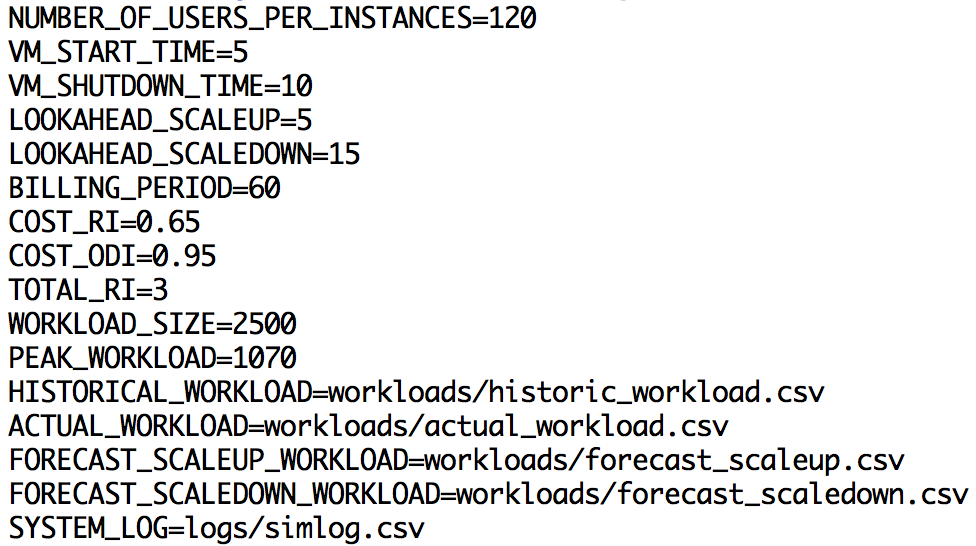
\includegraphics[scale=0.7]{simconfig.png}
    \caption{Simulation Configuration}
    \label{figure:simconfig}
  \end{center}
\end{figure}

\subsubsection{Output from ElasicSim}
\label{subs:Output from ElasicSim}
ElasicSim outputs are provided through logs and reports. Details of the logs generated, as comma separated value(csv) file, after each simulation run is provided here and the reports (PDF document) as output are discussed in evaluation section. ElasticSim provides two types of log files as output: VM usage logs and AppElastic logs. These two logs are as shown in the Figure~\ref{fig:elasticsimlogs}. These output is detailed as follows:
\begin{itemize}
  \item As shown in the Figure~\ref{figure:costlog}, VM usage log provides details about VM based on VM-ID. Billing hour start and Billing hour end fields are provided to identify the billing period of each VM. VM activity start and VM activity end fields are used to find in what period the VM was actively serving users. These time are recorded as Unix timestamps. VM usage time is recorded in Usage (in Minutes) field and the cost of using VM based the billing hours is recorded in Cost field.
  \item In Figure~\ref{figure:appelasticlogs}, logs related to AppElastic algorithm is shown. Its important to identify any anomaly in scaling algorithm, hence ElasticSim provides a detailed log of scaling. Logs are recorded for each time interval and helps in identifying the actual number of user request, number of VM's needed to serve these users and VM's provided by AppElastic algorithm. Each time interval is represented as unix timestamp in the field Unix timestamp. Actual number of users in the system is recorded in the field User request. Based on the threshold specified in the configuration and for the current number of user requests, VM required is recorded in VM needed field. VM activity such as billing start and activity start time are recorded VM active and VM billing fields respectively.
\end{itemize}
\begin{figure}
     \centering
     \begin{subfigure}[b]{1.0\textwidth}
         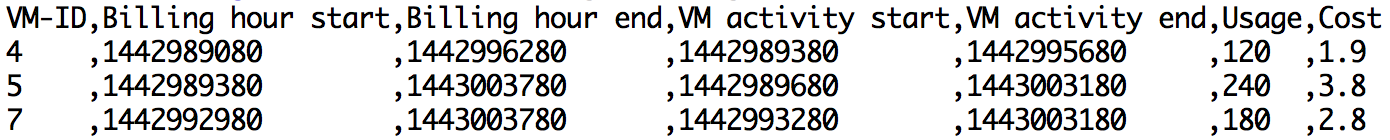
\includegraphics[width=\textwidth]{billinglog.png}
         \caption{VM usage log}
         \label{figure:costlog}
     \end{subfigure}
     \begin{subfigure}[b]{0.9\textwidth}
         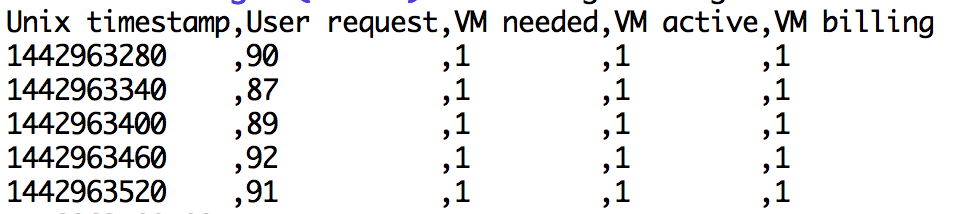
\includegraphics[width=\textwidth]{simlog.png}
         \caption{AppElastic logs}
         \label{figure:appelasticlogs}
     \end{subfigure}
     \caption{Output log from ElasticSim}
     \label{fig:elasticsimlogs}
 \end{figure}
 \section{Modeling workload \& prediction}
\label{sec:implementationprediction}
In this section implementation details of workload prediction is presented. ARIMA model discussed in the earlier chapter is applied to workload log trace and used for forecasting. Common obstacle for many while developing ARIMA model for forecasting is the selection of order of ARIMA process which considered as subjective and difficult task~\cite{makridakis2008forecasting}. Many years of research has gone into developing an automated approach to ARIMA model building. As introduced in the previous chapter, model building for ARIMA(p,d,q) process requires to choose values for p,d and q. Manual selection  of these parameter works if the input time series is know prior to building time series models. Since, the workload arriving to the system cannot be modeled easily there is a need for automating the model building. Solution to automated ARIMA model select process is given by Hyndman et al. ~\cite{hyndman2007automatic}. The algorithm guarantees to halt and return a valid model~\cite{hyndman2007automatic}. The selected model is used for forecasting. The algorithm by Hyndman et al~\cite{hyndman2007automatic} is implemented in a package called \(forecast\) in R software~\cite{rstat}. The implementation details of \(forecast\) library  and \(auto.arima()\) method are out of scope of this thesis. The function \(auto.arima()\) is used as black-box because the mechanism that transform the input workload into output model is obfuscated. A code snippet of forecasting workload for scale up is given in Listing~\ref{list:predscaleup}. For workload modeling reads the csv input workload trace and converts it into input time series data using R library called \(zoo\). In line number 5 and 6, the input timeseries data is divided into two parts. One for training and other for testing the model. The forecasted values are stored in \(arimaScaleupPrediction\) vector. The for loop in line 11 goes through the workload time series and starts building ARIMA model with the help of \(auto.arima()\) function. Since the training and testing datasets are on the same time scale, the for loop start from end of training dataset and runs until the end of the testing data. On the first iteration, first part of the workload i.e the training dataset is included into the model. On each iteration of the loop, new data points in the test dataset is included along with training data. Model building and forecasting is repeated every five minutes as specified in forecast\_interval. Actual forecasting of the data points is done in the line number 13. Forecasting is done with the help of a function called \(forecast\) and the forecast horizon is specified in horizon\_scaleup for scaleup. The forecast accuracy is recorded after every forecasting, and is recorded to a file as specified in line 14. Code snippet for predicting scale down time series is same as scale up prediction, but the only differing is in the horizon value which will be 15 minutes.
\begin{lstlisting}[language=R,caption=ARIMA Scaleup Model,label=list:predscaleup,numbers=left,frame=single,fontadjust=true,breaklines,basicstyle=\small]
workload=read.csv(WORKLOAD,sep=",",header=F);
workload_header=c("UnixTimeStamp","ActiveSessions");
colnames(workload) <- workload_header;
workload_tsdata=zoo(workload$ActiveSessions,workload$posxtime);
trainsamples=workloadsize/2;
testsamples=workloadsize/2;
#Forecast interval in minutes
forecast_interval=5;
#predict for scaleup
arimaScaleupPrediction=c();
for (i in seq(trainsamples,workloadsize,forecast_interval)){
  arimaFit=auto.arima(workload_tsdata[1:i])
  pred=forecast(arimaFit,h=horizon_scaleup)
  sink("accuracy_scaleup.log",append =T);
  print(accuracy(pred));
  sink();
  arimaScaleupPrediction=c(arimaScaleupPrediction,pred$mean);
}
\end{lstlisting}
Numerous error metrics have been proposed to capture the different between point forecast and corresponding observations. One of the most common forecast accuracy metric is based on mean square error (MSE)\cite{makridakis2008forecasting}. MSE is classify as scale dependent error metric. In the scope of this thesis, mean absolute percentage error (MAPE)\cite{makridakis2008forecasting}, which is a measure of prediction accuracy of forecasting model. MAPE is given by the formula:
\begin{equation}
  MAPE = 1/n \sum_{t=1}^{n} |\frac{A_{t}-F_{t}}{A_{t}}|
\end{equation}
where \(A_{t}\) is the actual value and \(F_{t}\) is the forecast value. The difference between \(A_{t}\) and \(F_{t}\) is then divided by the Actual value \(A_{t}\). The absolute value in this calculation is summed for every forecasted point in time and divided by the number of fitted points \(n\). Multiplying by 100 makes it a percentage error. Complete details of ARIMA model forecast accuracy is given evaluation section.
\section{AppElastic Algorithm Implementation}
\label{sec:AppElastic Algorithm Implementation}
In order to achieve the main research goal, that is to develop autoscaling algorithm, AppElastic algorithm is implemented in Java programming language. As said earlier AppElastic algorithm is a threshold based algorithm, it consist of three main internal parts as shown in the Figure~\ref{figure:appelasticparts}, and is described as follows:
\begin{itemize}
  \item Reader actual and predicted workloads: ElasticSim will guide the AppElastic algorithm in giving access to the log traces. ElasticSim generates the events for each entry in the log trace, accordingly AppElastic algorithm reads the Actual and predicted log traces to apply main algorithm logic.
  \item  Reading scaling thresholds configuration: The threshold information are as part of the ElasticSim configuration. AppElastic algorithm should read this threshold values to make the scaling decision.
  \item Generating scaling action using AppElastic Algorithm: Actual algorithm will run on the input data and generates the scaling actions.
\end{itemize}
\begin{figure}[h]
  \begin{center}
    \includegraphics[scale=0.7]{scaling.png}
    \caption{Parts of AppElastic}
    \label{figure:appelasticparts}
  \end{center}
\end{figure}
Since the autoscaling algorithm is implemented in a simulated environment, there will be no interaction between with any of the cloud service providers or any virtualization technologies. To support AppElastic algorithm each VM is modeled as an object. To model group of VM as resource pool, VM objects are grouped into Java list data structure. The object diagram is show in the Figure~\ref{figure:objdiag}.
\begin{figure}[h]
  \begin{center}
    \includegraphics[scale=0.7]{objdiag.png}
    \caption{AppElastic object diagram}
    \label{figure:objdiag}
  \end{center}
\end{figure}
The VM object will hold state related to virtual machine. Below is the details of the states presented in the VM object:
\begin{itemize}
  \item billingHourStart: As its was discussed in the previous chapter, taking Amazon AWS an example for cloud service provider, once the cloud user make a API call to cloud service provider the billing period start. To model this time, billingHourStart various holding unix timestamp is used.
  \item billingHourEnd: Once a machine is started based on the workload, VM will be shutdown or kept running. To track the VM billing period billingHourEnd variable is used. This is also a unix timestamp.
  \item startOfActivePeriod: As discussed before, after making call to cloud service API VM takes few mins to start. To model this,  startOfActivePeriod holds the unix time stamp of actual start of VM operation.
  \item endOfActivePeriod: Since the VM should be shutdown before the end of the billing period to avoid billing to next hour. This variable is used to hold the value to track ending of billing period.
  \item canExtend: Is a boolean variable which is used by AppElastic to logically shutdown the machine.
  \item machineID: To uniquely identify VM's for billing purpose.
\end{itemize}
AppElastic algorithm class maintains virtual machine as list of object. This is as depicted in the Figure~\ref{figure:objdiag}. For accountability AppElastic algorithm maintains different type of instances in two list. This is as described as:
\begin{itemize}
  \item runingRiInstances:This is a list of VmInstance type and this list contains the list of VMInstance which are as part of reserved instances.
  \item runningOdiInstances:This is a list of VmInstance type and this models the list of on demanded instances used as part of scaling.
\end{itemize}
Reserved instances and on-demand instances has different billing period requirements. Hence RI instances billing period will the entire life time of the simulation. And on-demand instances are billed as per the instance hour. As shown in the object diagram AppElastic object support two operations. The operation runAppElastic is implementation of AppElastic algorithm from Algorithm~\ref{algo:appelasticwithlookahead}, which does not differentiate between instance types such as reserved instances and on-demand stances. This operation is important in calculating the number of instances needed for a given workload which helps in finding right number of reserved instances.  This method is a generalization of the operation runAppElasticWithRi. The functionality of this operation can be divided into three parts:
\begin{itemize}
  \item scale up: Code snippet for this part is as shown in the Listing~\ref{list:appelasticscaleup}. In the first line, getRequestCountsInTimeRange is responsible for lookahead. It reads the predicted workload and returns the list of user request between the current time until the lookahead period. This list of user request is sorted to retrieve the maximum number users accommodate by the VM's. Based on this maximum number of user request, number of VM's required is calculated based on the specified threshold value.  For loop in line 6 is used to find if there are any running instances, this can be implied by the fact that, if a machine is in the active period then it running.
  Based on the number of machines required and machines running, if necessary new machines will be added through the for loop in line 12.  When a VM is created, it gets a new machine ID, the  billingHourStart get the value of current time,  billingHourEnd get the value of billing hour specified as unix timestamp.  StartOfActivePeriod takes the value of current time plus time taken to VM start as specified in configuration. EndOfActivePeriod takes the value based on the time taken to shutdown specified in configuration file.
  \item scale down:  Code snippet for this part is as shown in the Listing~\ref{list:appelasticscaledown}.  In the first line getRequestCountsInTimeRange is responsible for lookahead. It reads the predicted workload and returns the list of user request between the current time until the lookahead period for scale down. This list of user request is sorted to retrieve the maximum number users accommodate by the VM's. Based on this maximum number of user request, number of VM's required for next billing hours is calculated based on the specified threshold value. One of the main idea behind AppElastic algorithm is killing of the VM's only at the end of the billing cycle. Once the number of machine to shutdown is calculated, the VM's which are ending billing period are identified in the for loop at line 6. If the number of machines required in the next billing period is less than the machines ending billing period then all the VM's ending the billing period is shutdown. This is done in the for loop at line 13. And if the machines required in the next billing cycle is less than number of VM's ending its billing period, then only  a subset of VM's is shutdown. This is done through the loop at line 19.  As said before VM's shutdown is modeled by setting boolean value canExtent at line 23.
  \item Noscale / extend VM:  Code snippet for this part is as shown in the Listing~\ref{list:appelasticnoscale}.  In the case of no scaling action is taken, it either means the machines are killed or the machines which are running should be kept running for next billing period. This is done by finding the machines which are ending the billing period and extending to the next billing period by setting endOfActtivePeriod and billingHourEndTime. This is achieved in the for loop block in the first line.
\end{itemize}
The second operation is implemented as shown in the listing. Main difference between to runAppElastic method is that, it differentiate between reserved instances and on-demand instances. The reserved instances are never shutdown and its kept running until the end of simulation.
\begin{lstlisting}[language=java,caption=AppElastic Scaleup,label=list:appelasticscaleup,numbers=left,frame=single,fontadjust=true,breaklines,basicstyle=\small]
ArrayList<Integer> userInPredictedInterval=getRequestCountsInTimeRange(timeStamp, timeStamp + scaleUpLookAhead,false);
Collections.sort(userInPredictedInterval);
int maxUserIntervalPredicted=userInPredictedInterval.get(userInPredictedInterval.size() - 1);
int machineReq=(int)Math.ceil((double)maxUserIntervalPredicted/numberOfUserPerInstance);
int machineRunning = 0;
for (int i = 0;i < runningInstance.size();i++) {
 if(timeStamp<=runningInstance.get(i).endOfActivePeriod)
  machineRunning+=1;
}
if (machineReq>machineRunning) {
 int machinesToAdd=machineReq-machineRunning;
 for (int i=0;i<machinesToAdd;i++) {
  machineID+=1;
  runningInstance.add(new VmInstance(machineID,timeStamp,timeStamp+billingPeriod,timeStamp+timeTakenToActive, (timeStamp+billingPeriod)-timetakenToShutdown));
 }
}
\end{lstlisting}
\begin{lstlisting}[language=java,caption=AppElastic Scaledown,label=list:appelasticscaledown,numbers=left,frame=single,fontadjust=true,breaklines,basicstyle=\small]
ArrayList<Integer> usersInIntervalPredictedForScaleDown=getRequestCountsInTimeRange(timeStamp,timeStamp+ scaleDownLookAhead,true);
Collections.sort(usersInIntervalPredictedForScaleDown);
int maxUserIntervalPredictedScaleDown=usersInIntervalPredictedForScaleDown.get(usersInIntervalPredictedForScaleDown.size()-1);
int machineRequired=(int)Math.ceil((double)maxUserIntervalPredictedScaleDown/numberOfUserPerInstance);
ArrayList<VmInstance> vmsEndingActivePeriod = new ArrayList<>();
for (int i=0;i<runningInstance.size();i++) {
	if (runningInstance.get(i).endOfActivePeriod==timeStamp)
		vmsEndingActivePeriod.add(runningInstance.get(i));
}
int totalVmToKill=machineRunning-machineRequired;
// kill all vm's which are ending active period.
if ( totalVmToKill>=vmsEndingActivePeriod.size() ) {
 for (int j=0;j<vmsEndingActivePeriod.size();j++)
  for (int i=0;i<runningInstance.size();i++)
   if (runningInstance.get(i).machineID==vmsEndingActivePeriod.get(j).machineID)
    runningInstance.get(i).canExtend=false;
}
// kill only subset of vm's ending active period.
if (totalVmToKill<vmsEndingActivePeriod.size()) {
 for (int j=0;j<totalVmToKill;j++) {
  for (int i=0;i<runningInstance.size();i++) {
   if (runningInstance.get(i).machineID==vmsEndingActivePeriod.get(j).machineID)
    runningInstance.get(i).canExtend=false;
	 }
	}
}
\end{lstlisting}
\begin{lstlisting}[language=java,caption=AppElastic No scale/extend VM,label=list:appelasticnoscale,numbers=left,frame=single,fontadjust=true,breaklines,basicstyle=\small]
for (int i=0;i<runningInstance.size();i++) {
 if (timeStamp==runningInstance.get(i).endOfActivePeriod && runningInstance.get(i).canExtend) {
  runningInstance.get(i).endOfActivePeriod+=billingPeriod;
  runningInstance.get(i).billingHourEndTime+=billingPeriod;
 }
}
\end{lstlisting}

\section{Evaluation}
\label{sec:Evaluation}
This section presents results evaluating AppElastic algorithm and ARIMA forecast model. At first evaluation of AppElastic Algorithm is presented in Section~\ref{sub:Evaluation of AppElastic Algorithm}. In section~\ref{sub:Forecast Accuracy} accuracy of ARIMA forecast model is discussed. The results of SLA violation due to forecast error is discussed in the section~\ref{sub:SLA violation}. Cost is evaluated with a baseline price in Section~\ref{sub:Cost Evaluation}, and this is important to show how cost can be reduced by using AppElastic algorithm for resource planning and allocation. The data used in this study is acquired from Audio/Video conferencing application at Citrix Inc. Dresden as shown in the Figure~\ref{figure:workloadforsim}. Fixed experiment parameters which are necessary for execution of AppElastic algorithm and ElasticSim simulator are given in the Table~\ref{table:exppara}. These parameters are necessary as discussed in the section~\ref{sec:AppElastic Algorithm}.
\begin{center}
  \begin{table}
    \scalebox{1}{
    \begin{tabular}{ | L{8cm} | L{6cm} |}
      \hline
      Parameter & Description \\ \hline
      NUMBER\_OF\_USERS\_PER\_INSTANCES & 120 users per instance \\ \hline
      VM\_START\_TIME & 5 minutes \\ \hline
      VM\_SHUTDOWN\_TIME & 10 minutes  \\ \hline
      LOOKAHEAD\_SCALEUP & 5 minutes\\ \hline
      LOOKAHEAD\_SCALEDOWN & 15 minutes\\ \hline
      BILLING\_PERIOD & 60 minutes\\ \hline
      COST\_RI & \$0.65 (USD)\\ \hline
      COST\_ODI & \$0.95 (USD) \\ \hline
    \end{tabular}
    }
    \caption{ Fixed experiment parameters}
     \label{table:exppara}
\end{table}
\end{center}
\begin{figure}[h]
  \begin{center}
    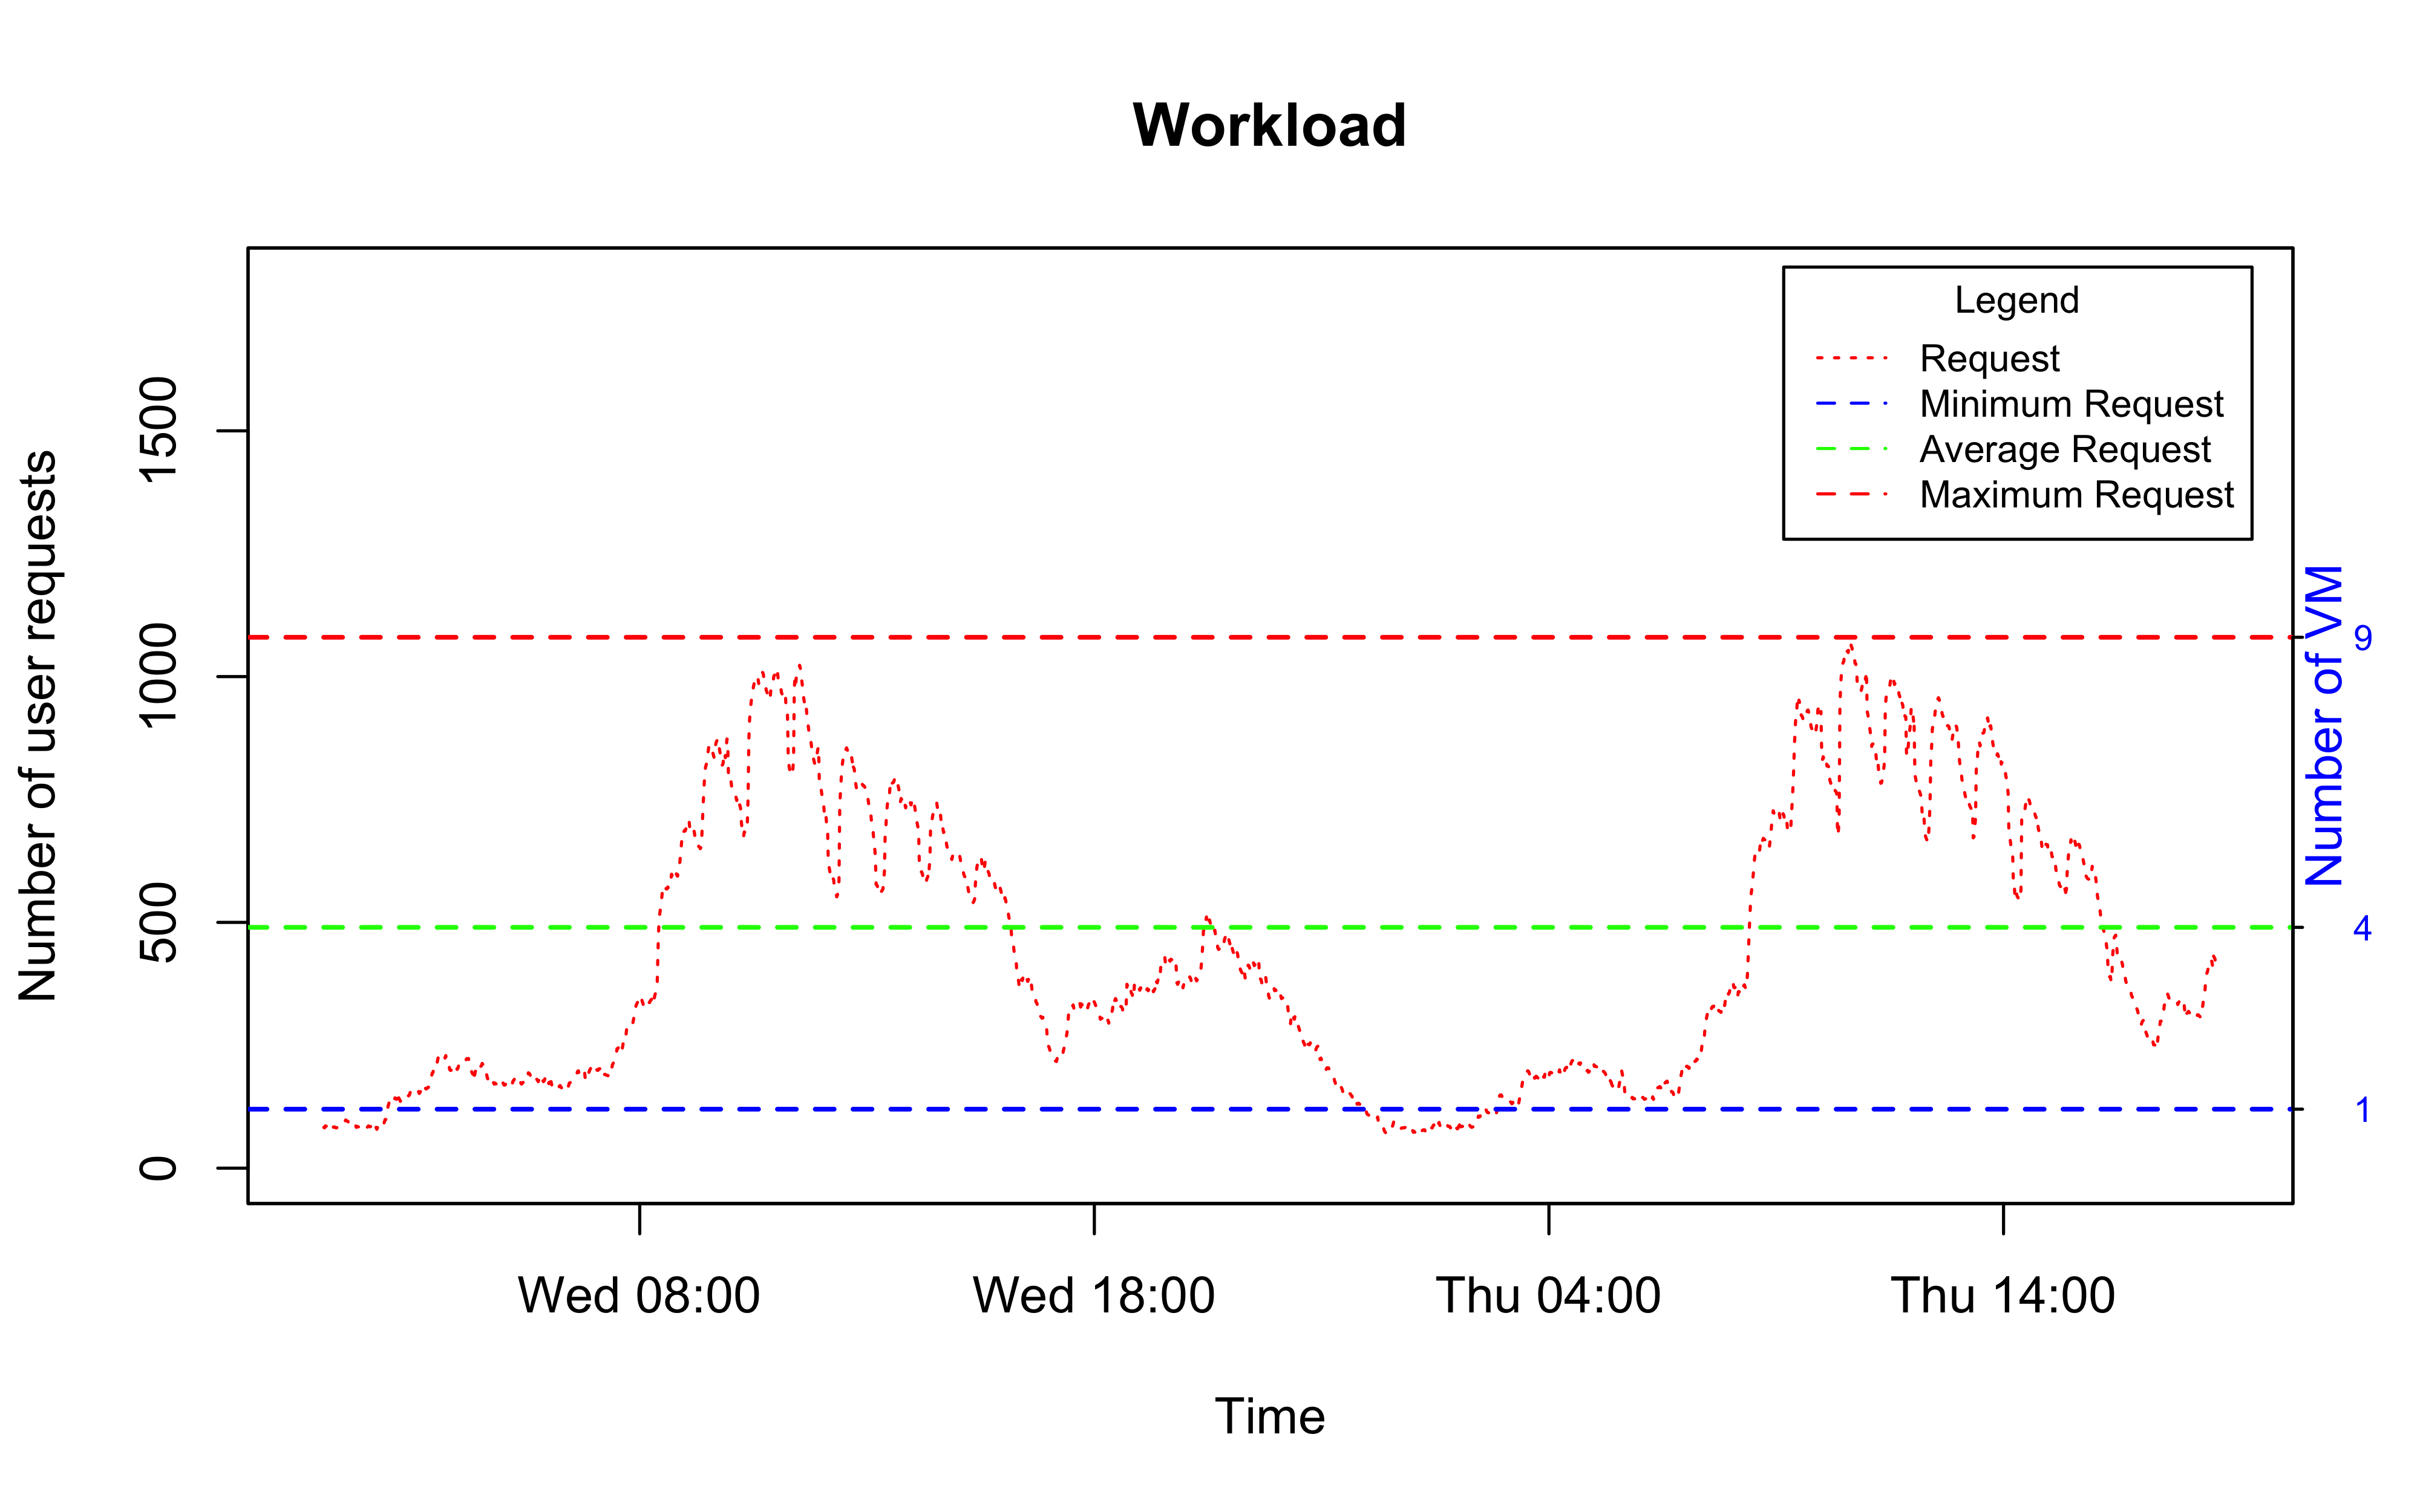
\includegraphics[scale=0.1]{workloadforsim.png}
    \caption{Workload for evaluation}
    \label{figure:workloadforsim}
  \end{center}
\end{figure}
\begin{figure}[h]
  \begin{center}
    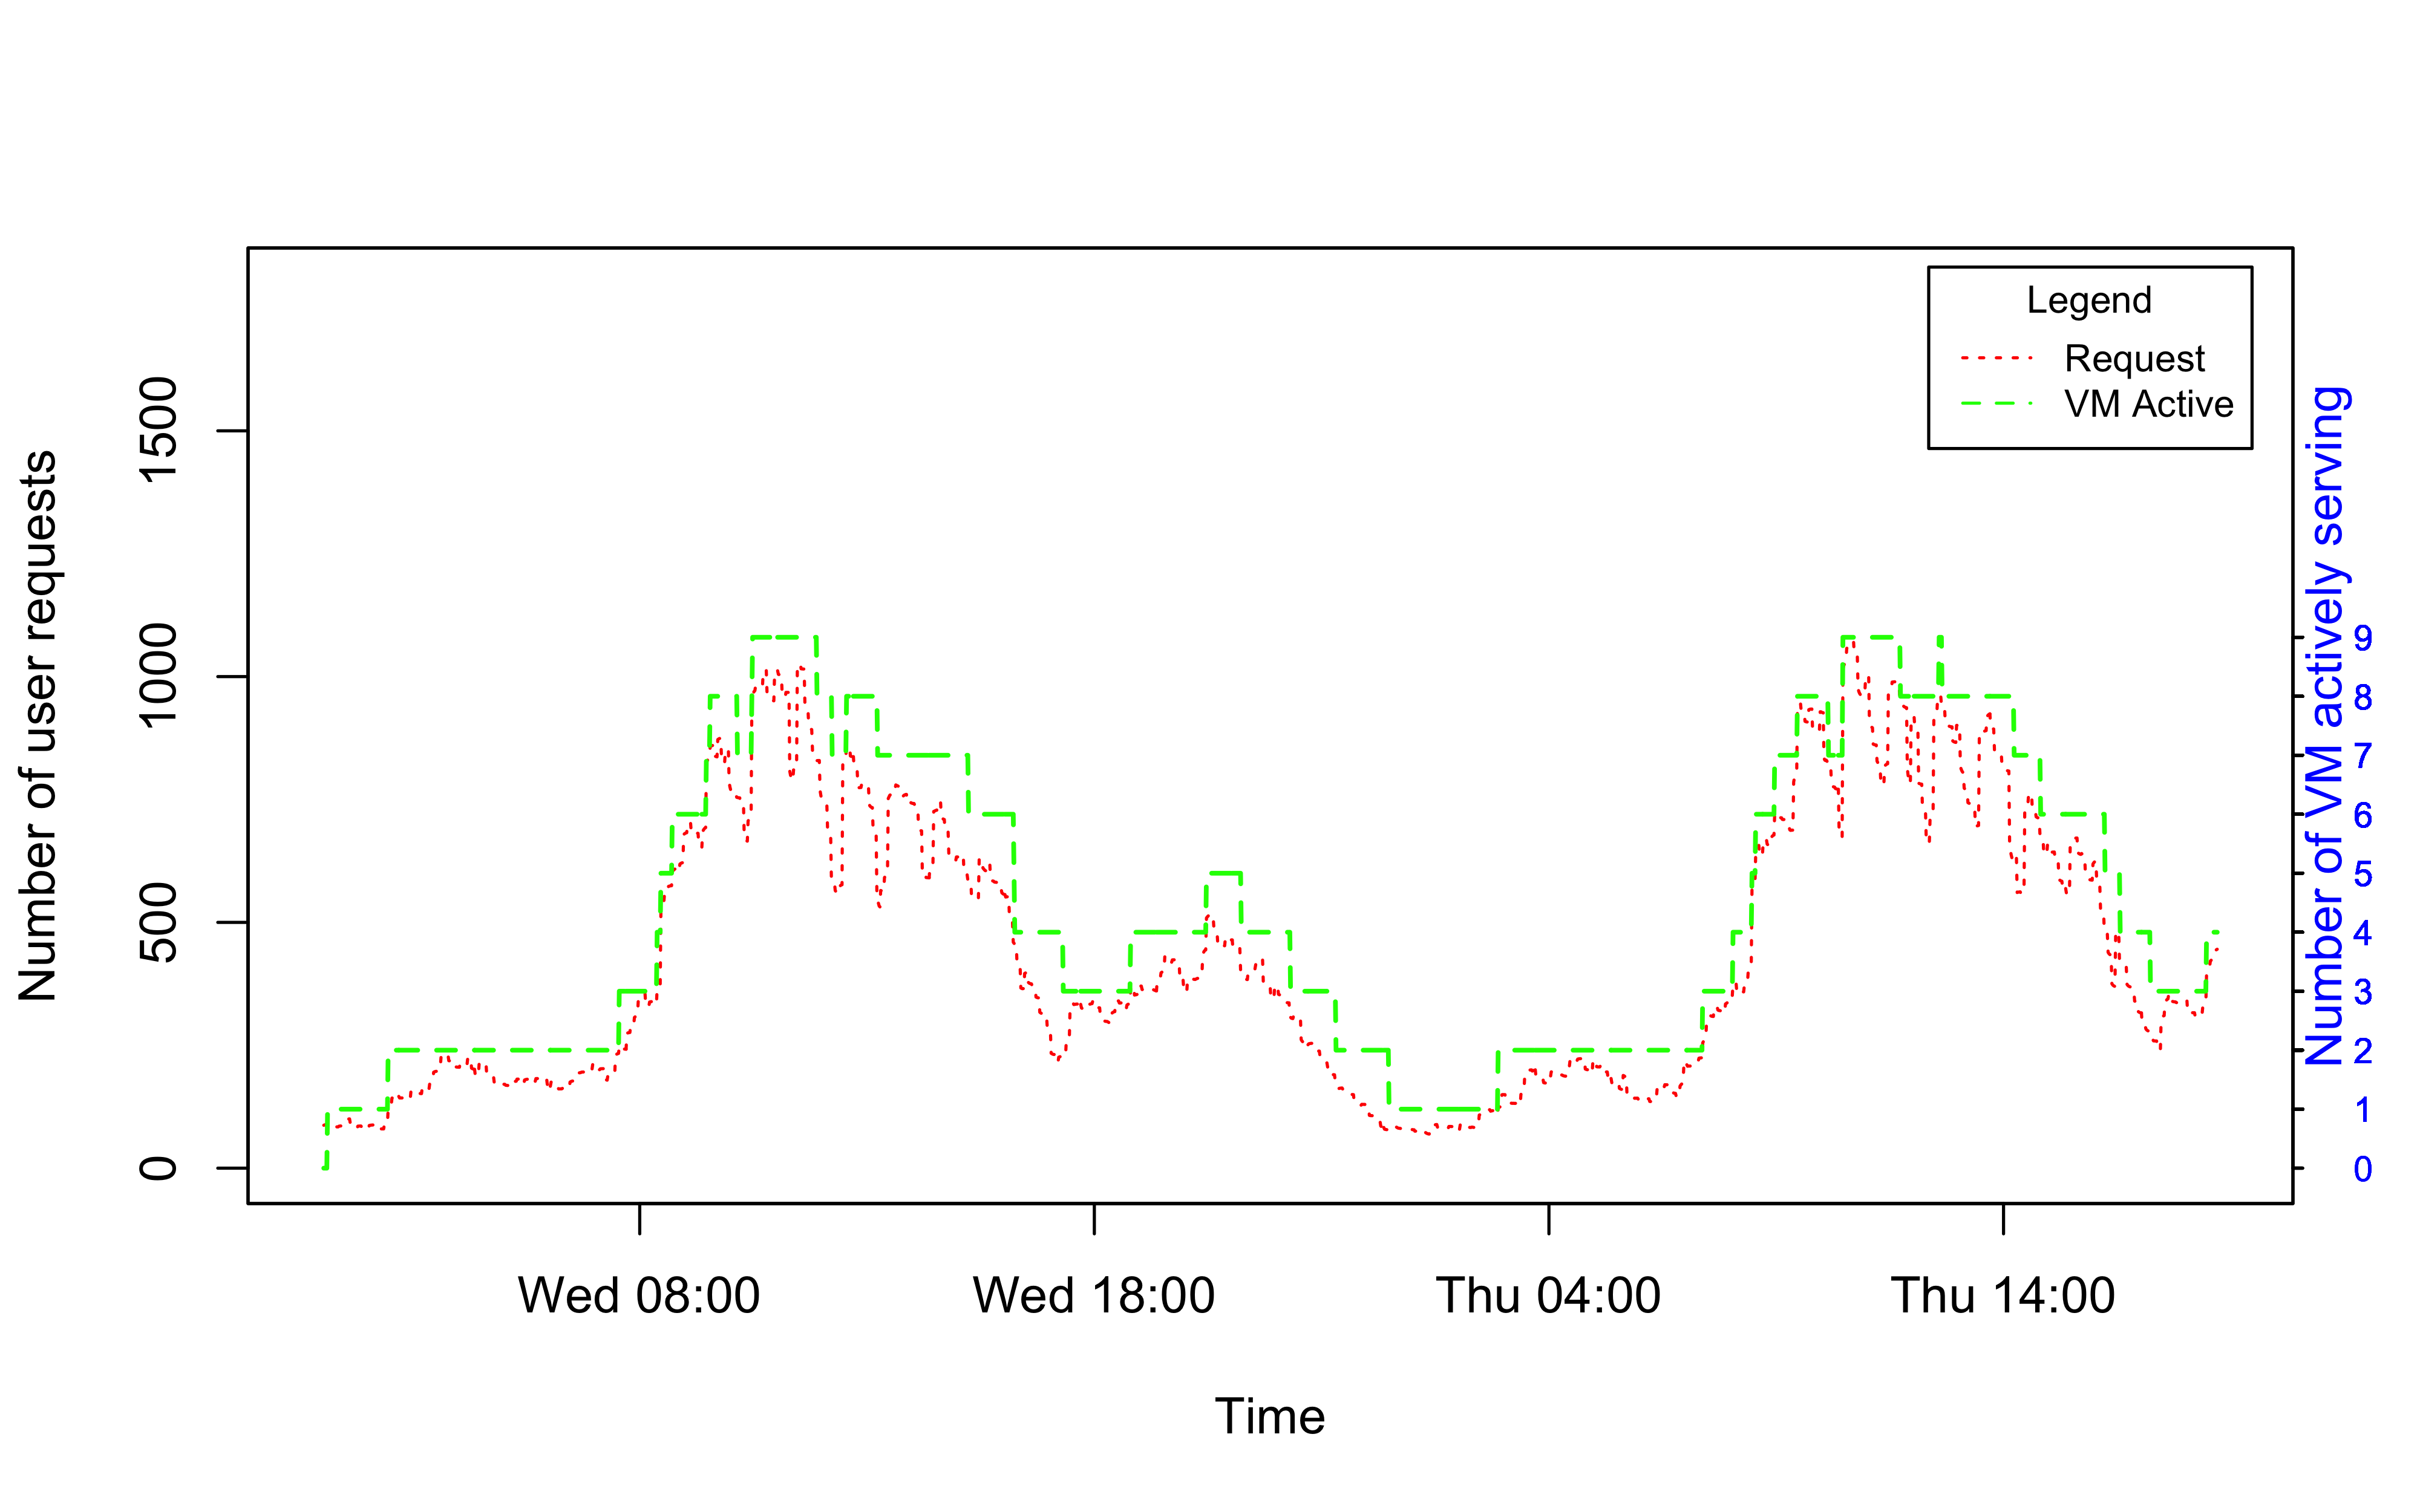
\includegraphics[scale=0.1]{highlevelvmscaling.png}
    \caption{AppElastic applied on input workload}
    \label{figure:appelasticapplication}
  \end{center}
\end{figure}
\subsection{Evaluation of AppElastic Algorithm}
\label{sub:Evaluation of AppElastic Algorithm}
A very important property to defined when a new algorithm is introduced is its correctness. To assert an algorithm is correct it should perform the task as per the specified requirements. To identify a mathematical model as correctness proof is out of scope of this thesis. However, its important to defined the correctness condition for finding the correctness of the algorithm. These correctness conditions will help in identifying any anomaly in the scaling algorithm. For AppElastic algorithm correctness condition can be defined as follows:
\begin{itemize}
  \item On correct execution of the AppElastic algorithm, each VM will be active after some time \(T\) as defined by VM startup time. In other words, the billing period start of the VM should be before its actual start. When a VM is shutdown, it take some time \(T\) as defined by VM shutdown time. Hence, when VM is shutdown at \(T_{i}\) then it will be stopped billing at time \(T_{i}\) + VM shutdown time. These both conditions can be proved by the log entries and plotting graphs from these data as provided by ElasticSim.
  \item Each VM has capacity of serving \(N\) number of user as specified in the \(numberOfUserPerInstance\) config option. If there are \(M\) number of users at time \(T\), the number of VM's active at time \(T\) should have the capacity to handle \(M\) users at time \(T\). And this capacity is given by the formula:
  \begin{equation}
    Capaticy_{t} = VM Active_{T} * \textrm{numberOfUsersPerInstance}
  \end{equation}
\end{itemize}
On the correct execution of AppElastic algorithm, above said conditions has to be fulfilled. To show whether AppElastic meets the first condition, Figure~\ref{figure:billingactivescaleup} and Figure~\ref{figure:billingactivescaledown} are presented. In these figures red dotted lines represents the input workload trace, blue line show VM's which are billing and green line shows these VM's which are active for user request. From Figure~\ref{figure:billingactivescaleup} its evident that AppElastic algorithm consider the delay in starting the VM. As its shows, VM's starts billing at 01:02 hours and VM will be active to serve users 5 minutes after at time 01:07 hours. Similarly, from Figure~\ref{figure:billingactivescaledown} its also evident that AppElastic algorithm consider the delay in shutting down of VM's. As shown, VM's stops being active for users at 11:52 hours and VM will ends billing at 12:02 hours.
\\
Figure~\ref{figure:appelasticapplication} shows how VM's are scaled up/down based on the variation in the workload. Red dotted lines represents the input workload trace and the green line show the capacity of active VM's serving the workload. Axis on the right hand side denotes the number of VM's being actively serving these request. From the Figures~\ref{fig:appelasticperformance} its evident that AppElastic algorithm allocates enough VM's in any rapidly changing user requests.
\begin{figure}
     \centering
     \begin{subfigure}[b]{1.0\textwidth}
         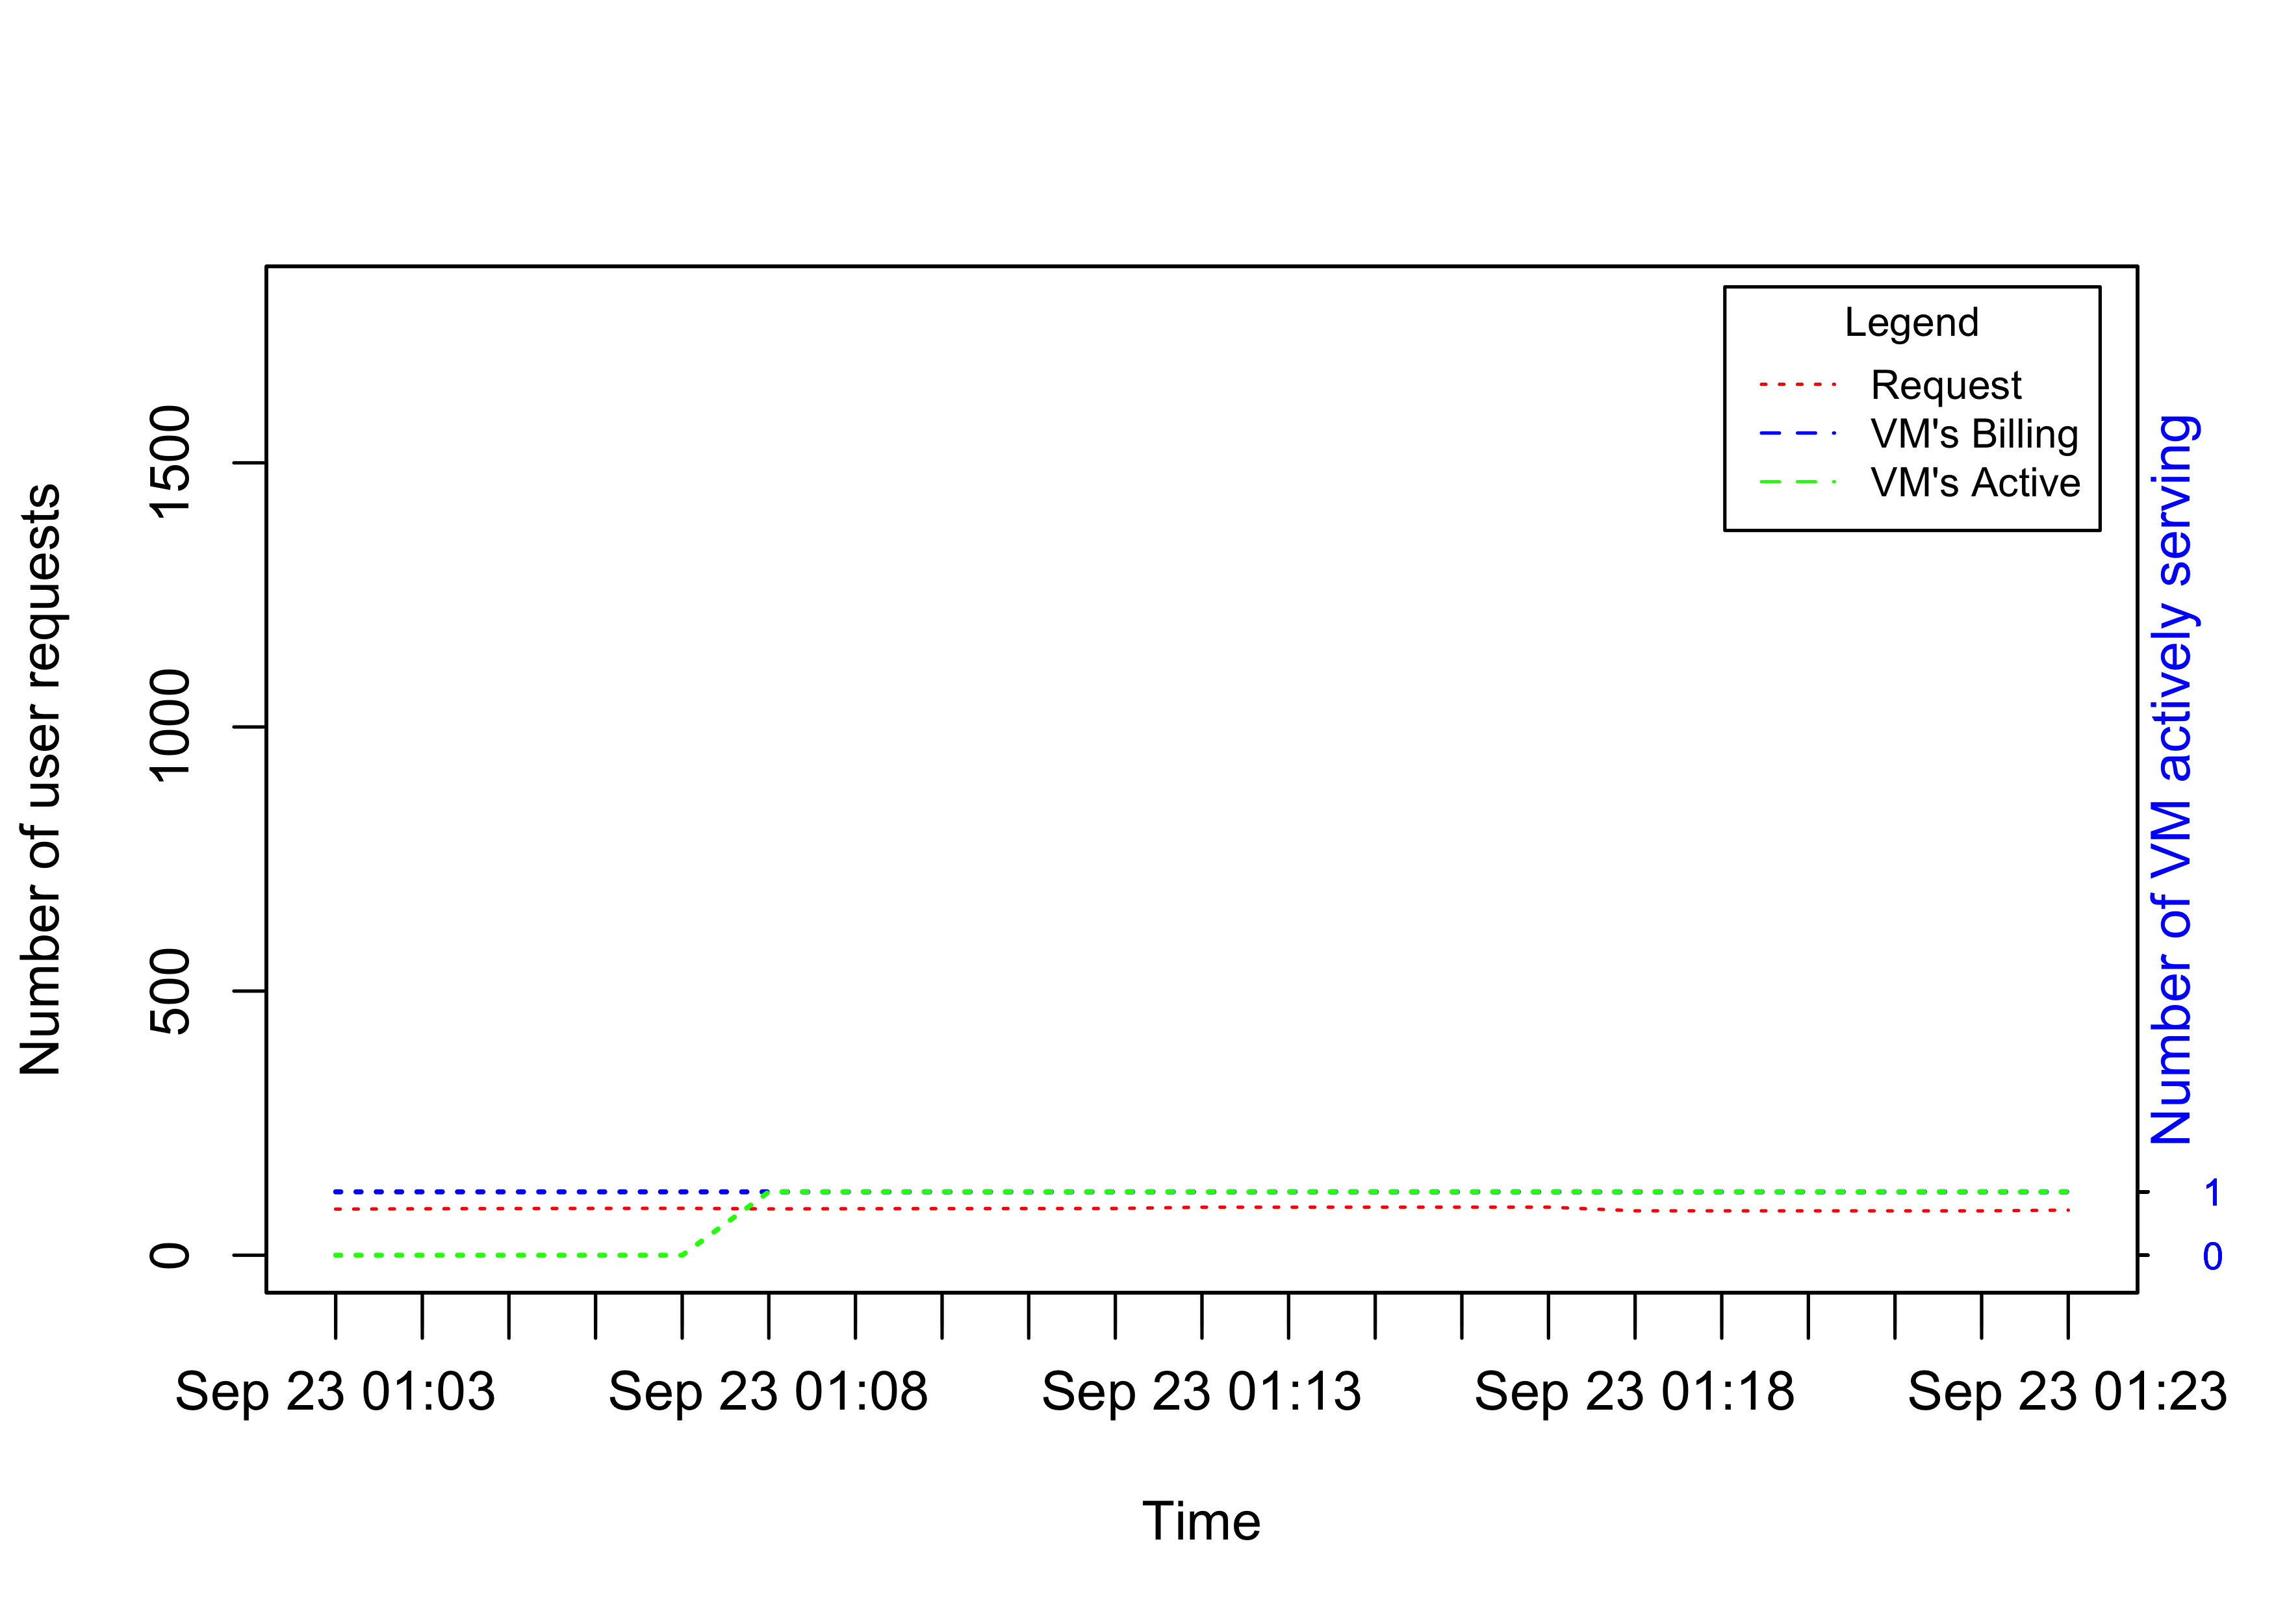
\includegraphics[width=\textwidth]{autoscalingdiagscaleup.png}
         \caption{Scale up: Showing time delay for VM to be active}
         \label{figure:billingactivescaleup}
     \end{subfigure}
     \begin{subfigure}[b]{0.9\textwidth}
         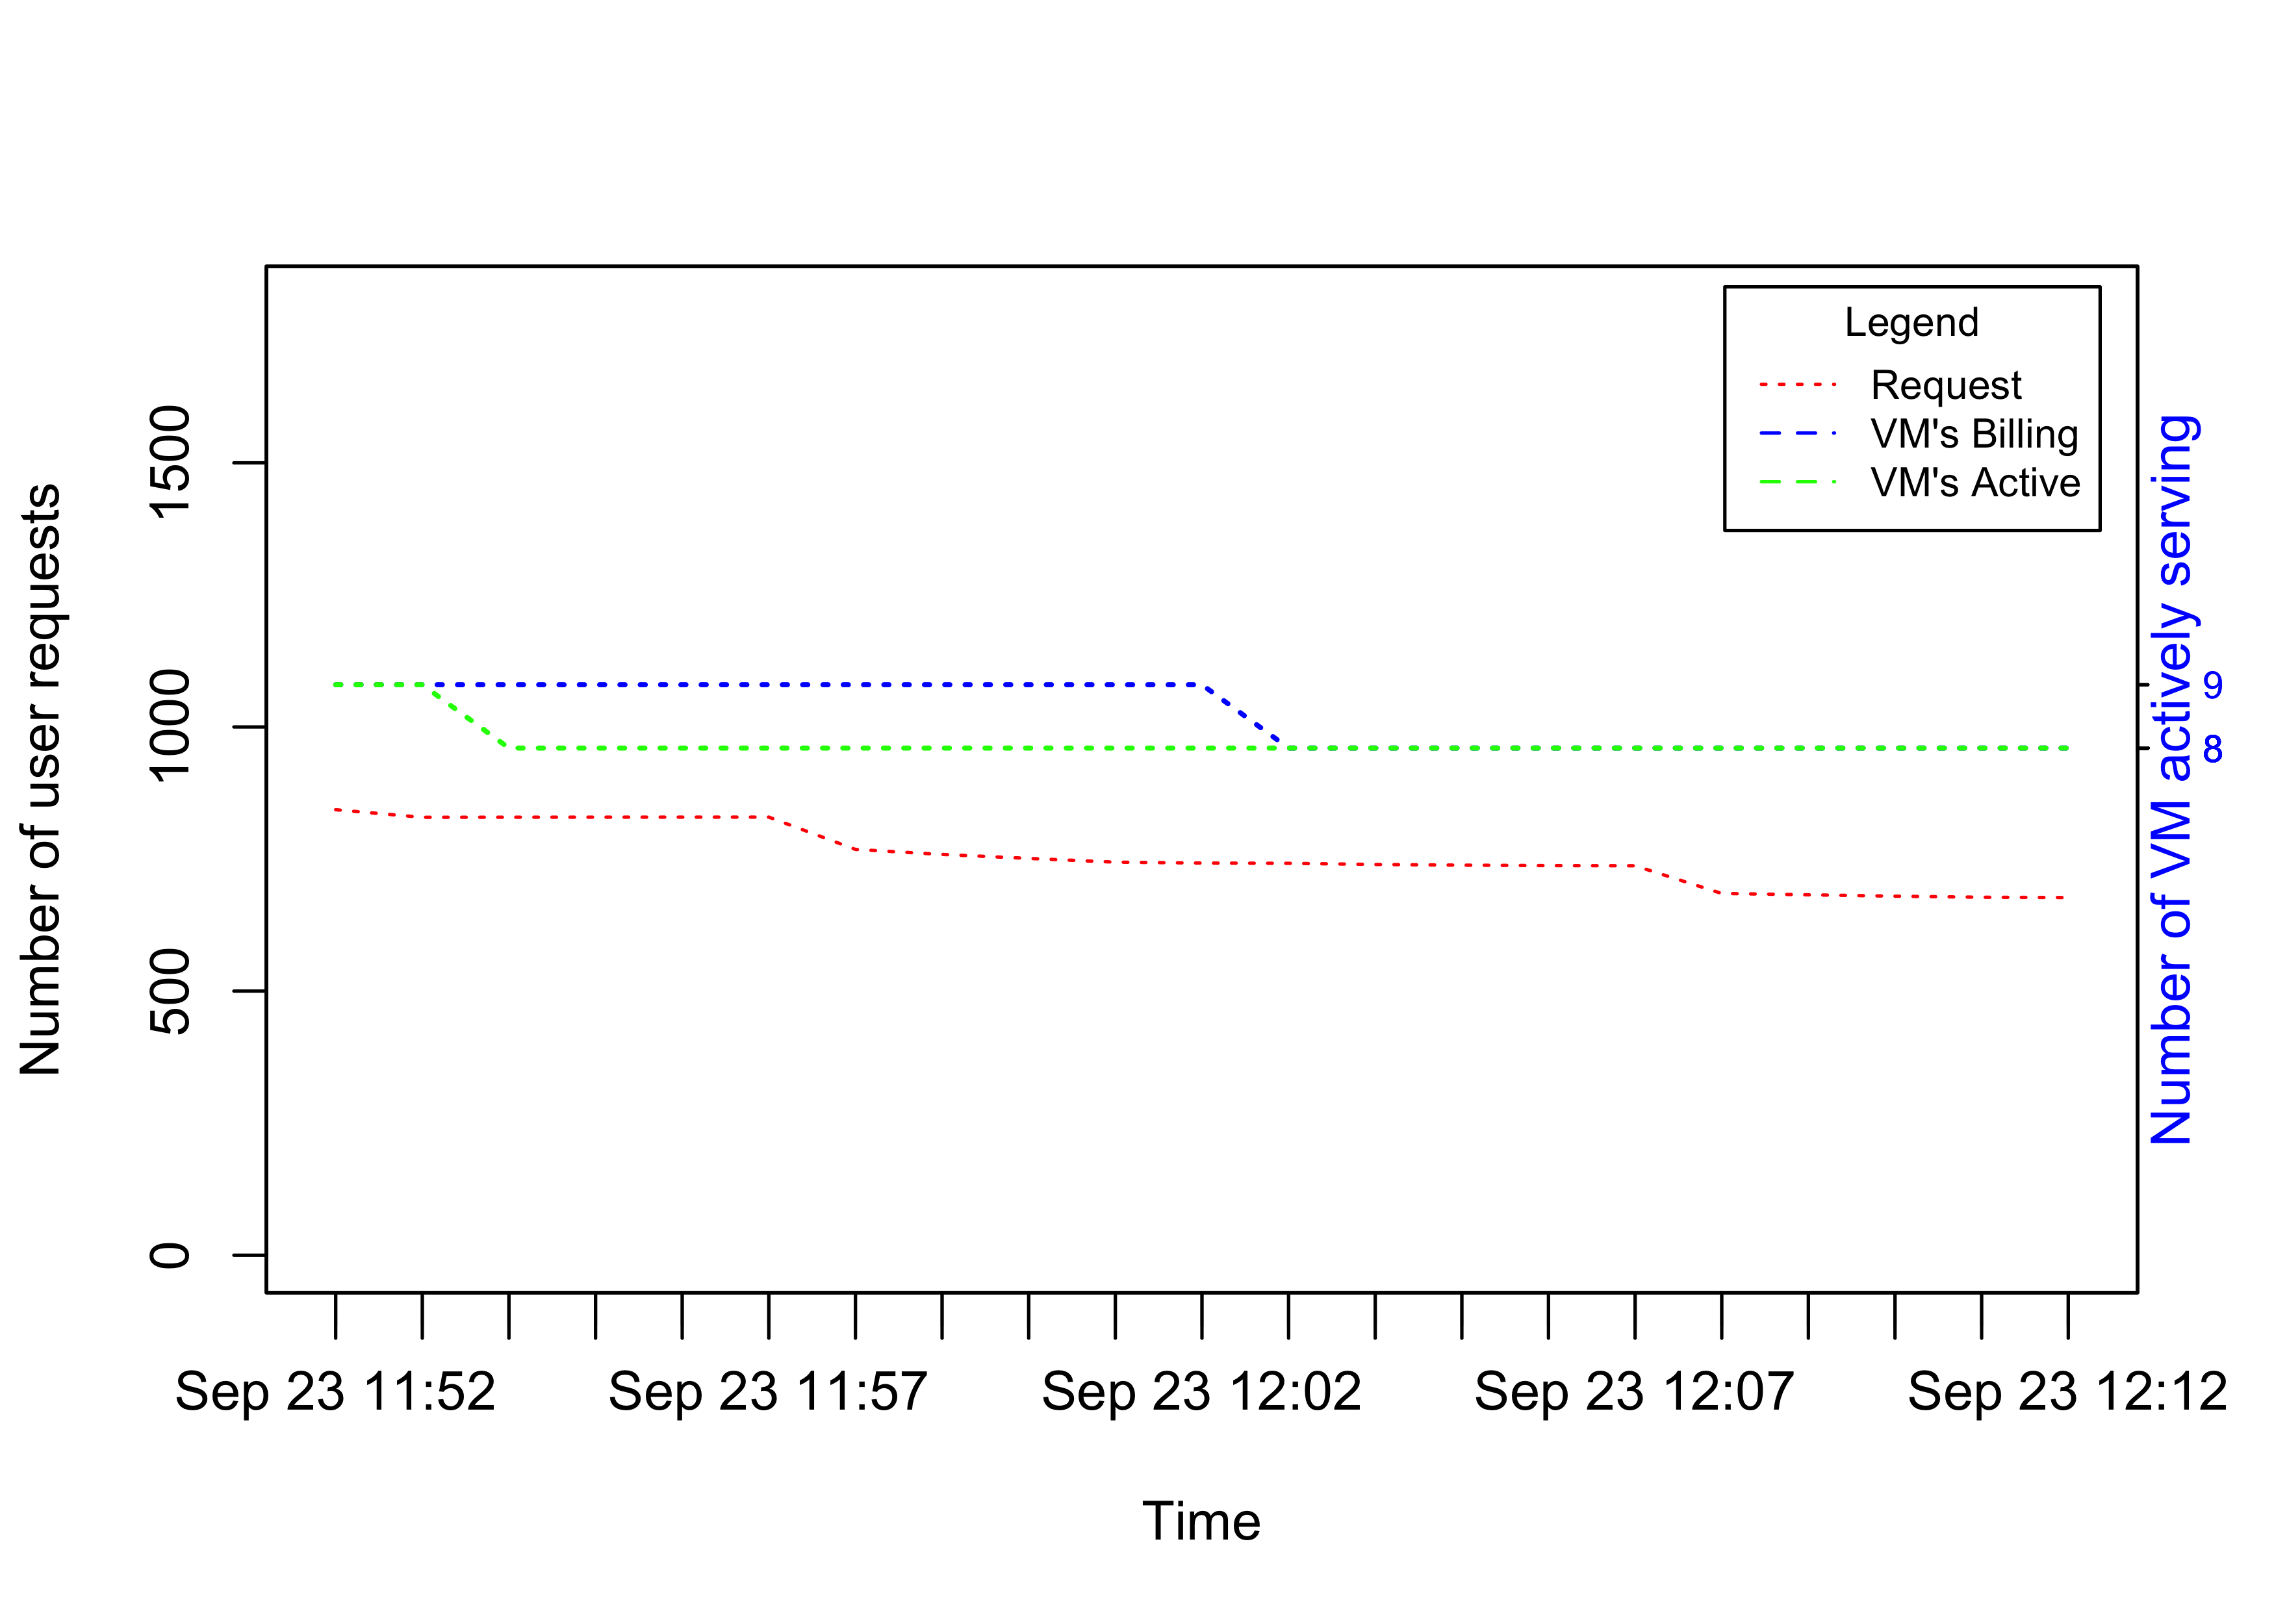
\includegraphics[width=\textwidth]{autoscalingdiagscaledown.png}
         \caption{Scale down: Showing time delay for VM to end billing}
         \label{figure:billingactivescaledown}
     \end{subfigure}
     \caption{Scale Up and Down}
     \label{fig:billingactive}
\end{figure}

\begin{figure}
     \centering
     \begin{subfigure}[b]{0.4\textwidth}
         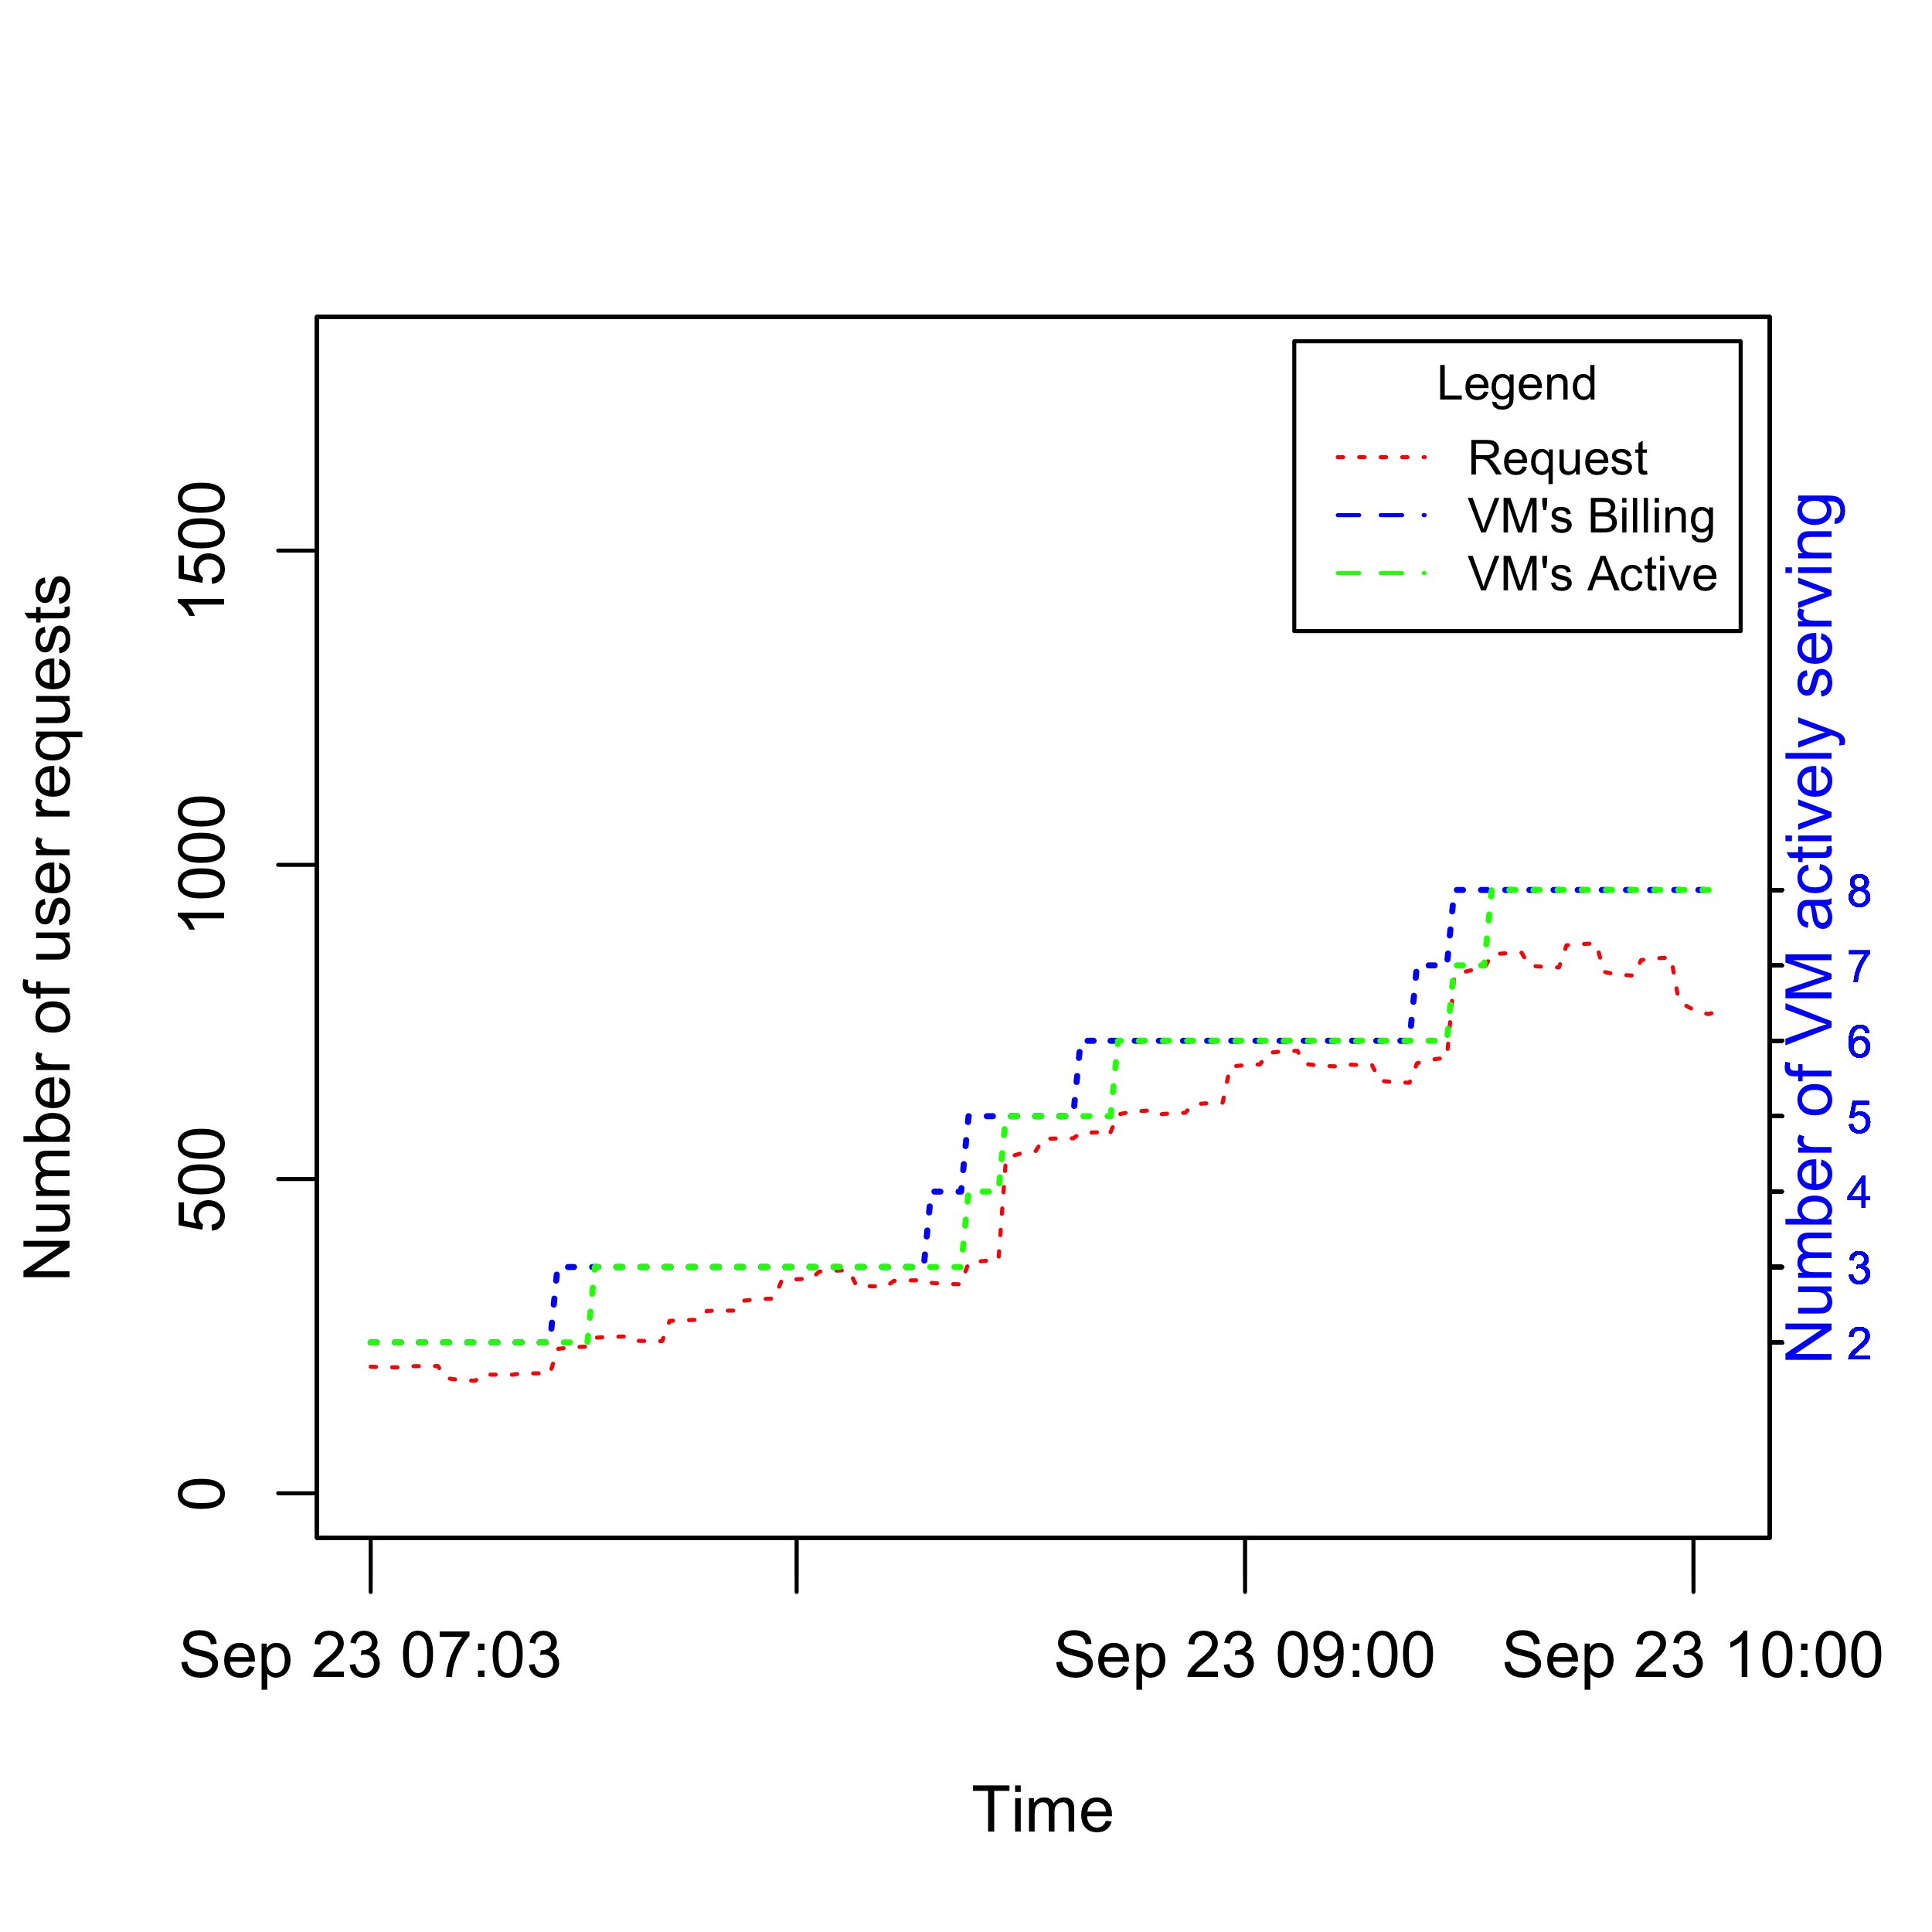
\includegraphics[width=\textwidth]{autoscalingdiag1.png}
         \caption{Increase in user request}
         \label{figure:autoscalingdiag1}
     \end{subfigure}
      \hfill
     \begin{subfigure}[b]{0.4\textwidth}
         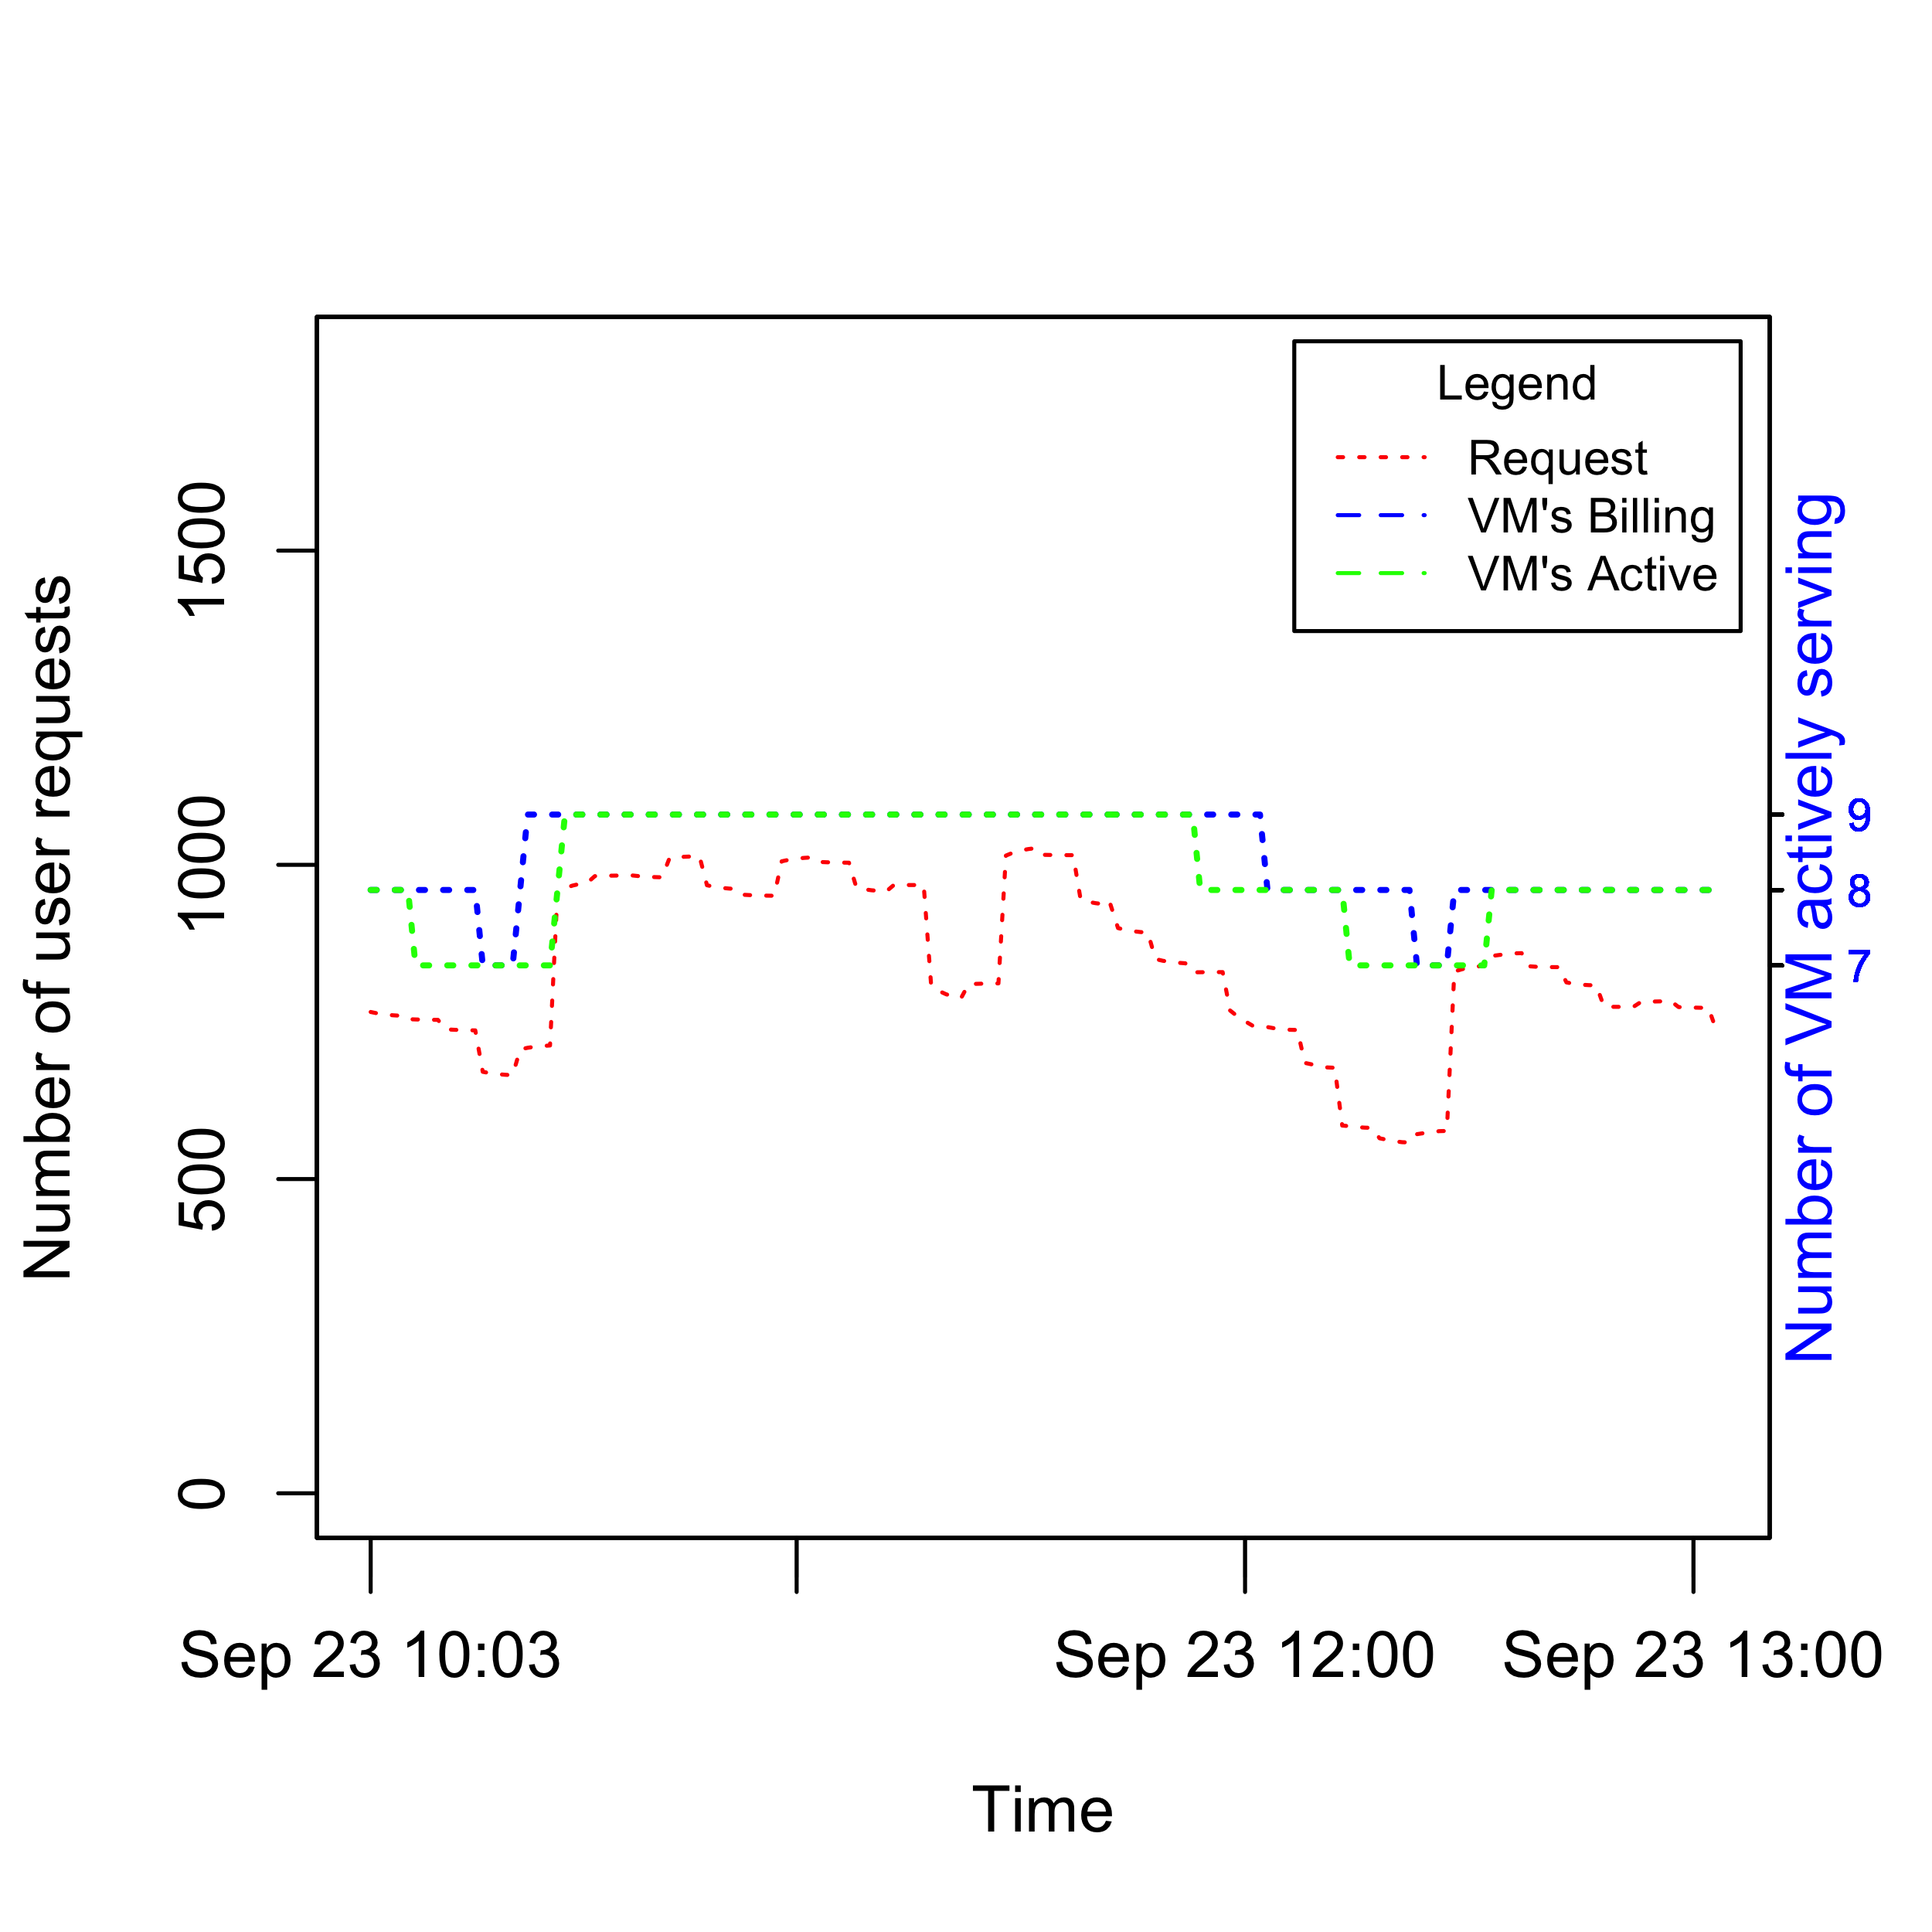
\includegraphics[width=\textwidth]{autoscalingdiag2.png}
         \caption{Rapid change in user request}
         \label{figure:autoscalingdiag2}
     \end{subfigure}
     \vskip\baselineskip
     \begin{subfigure}[b]{0.4\textwidth}
         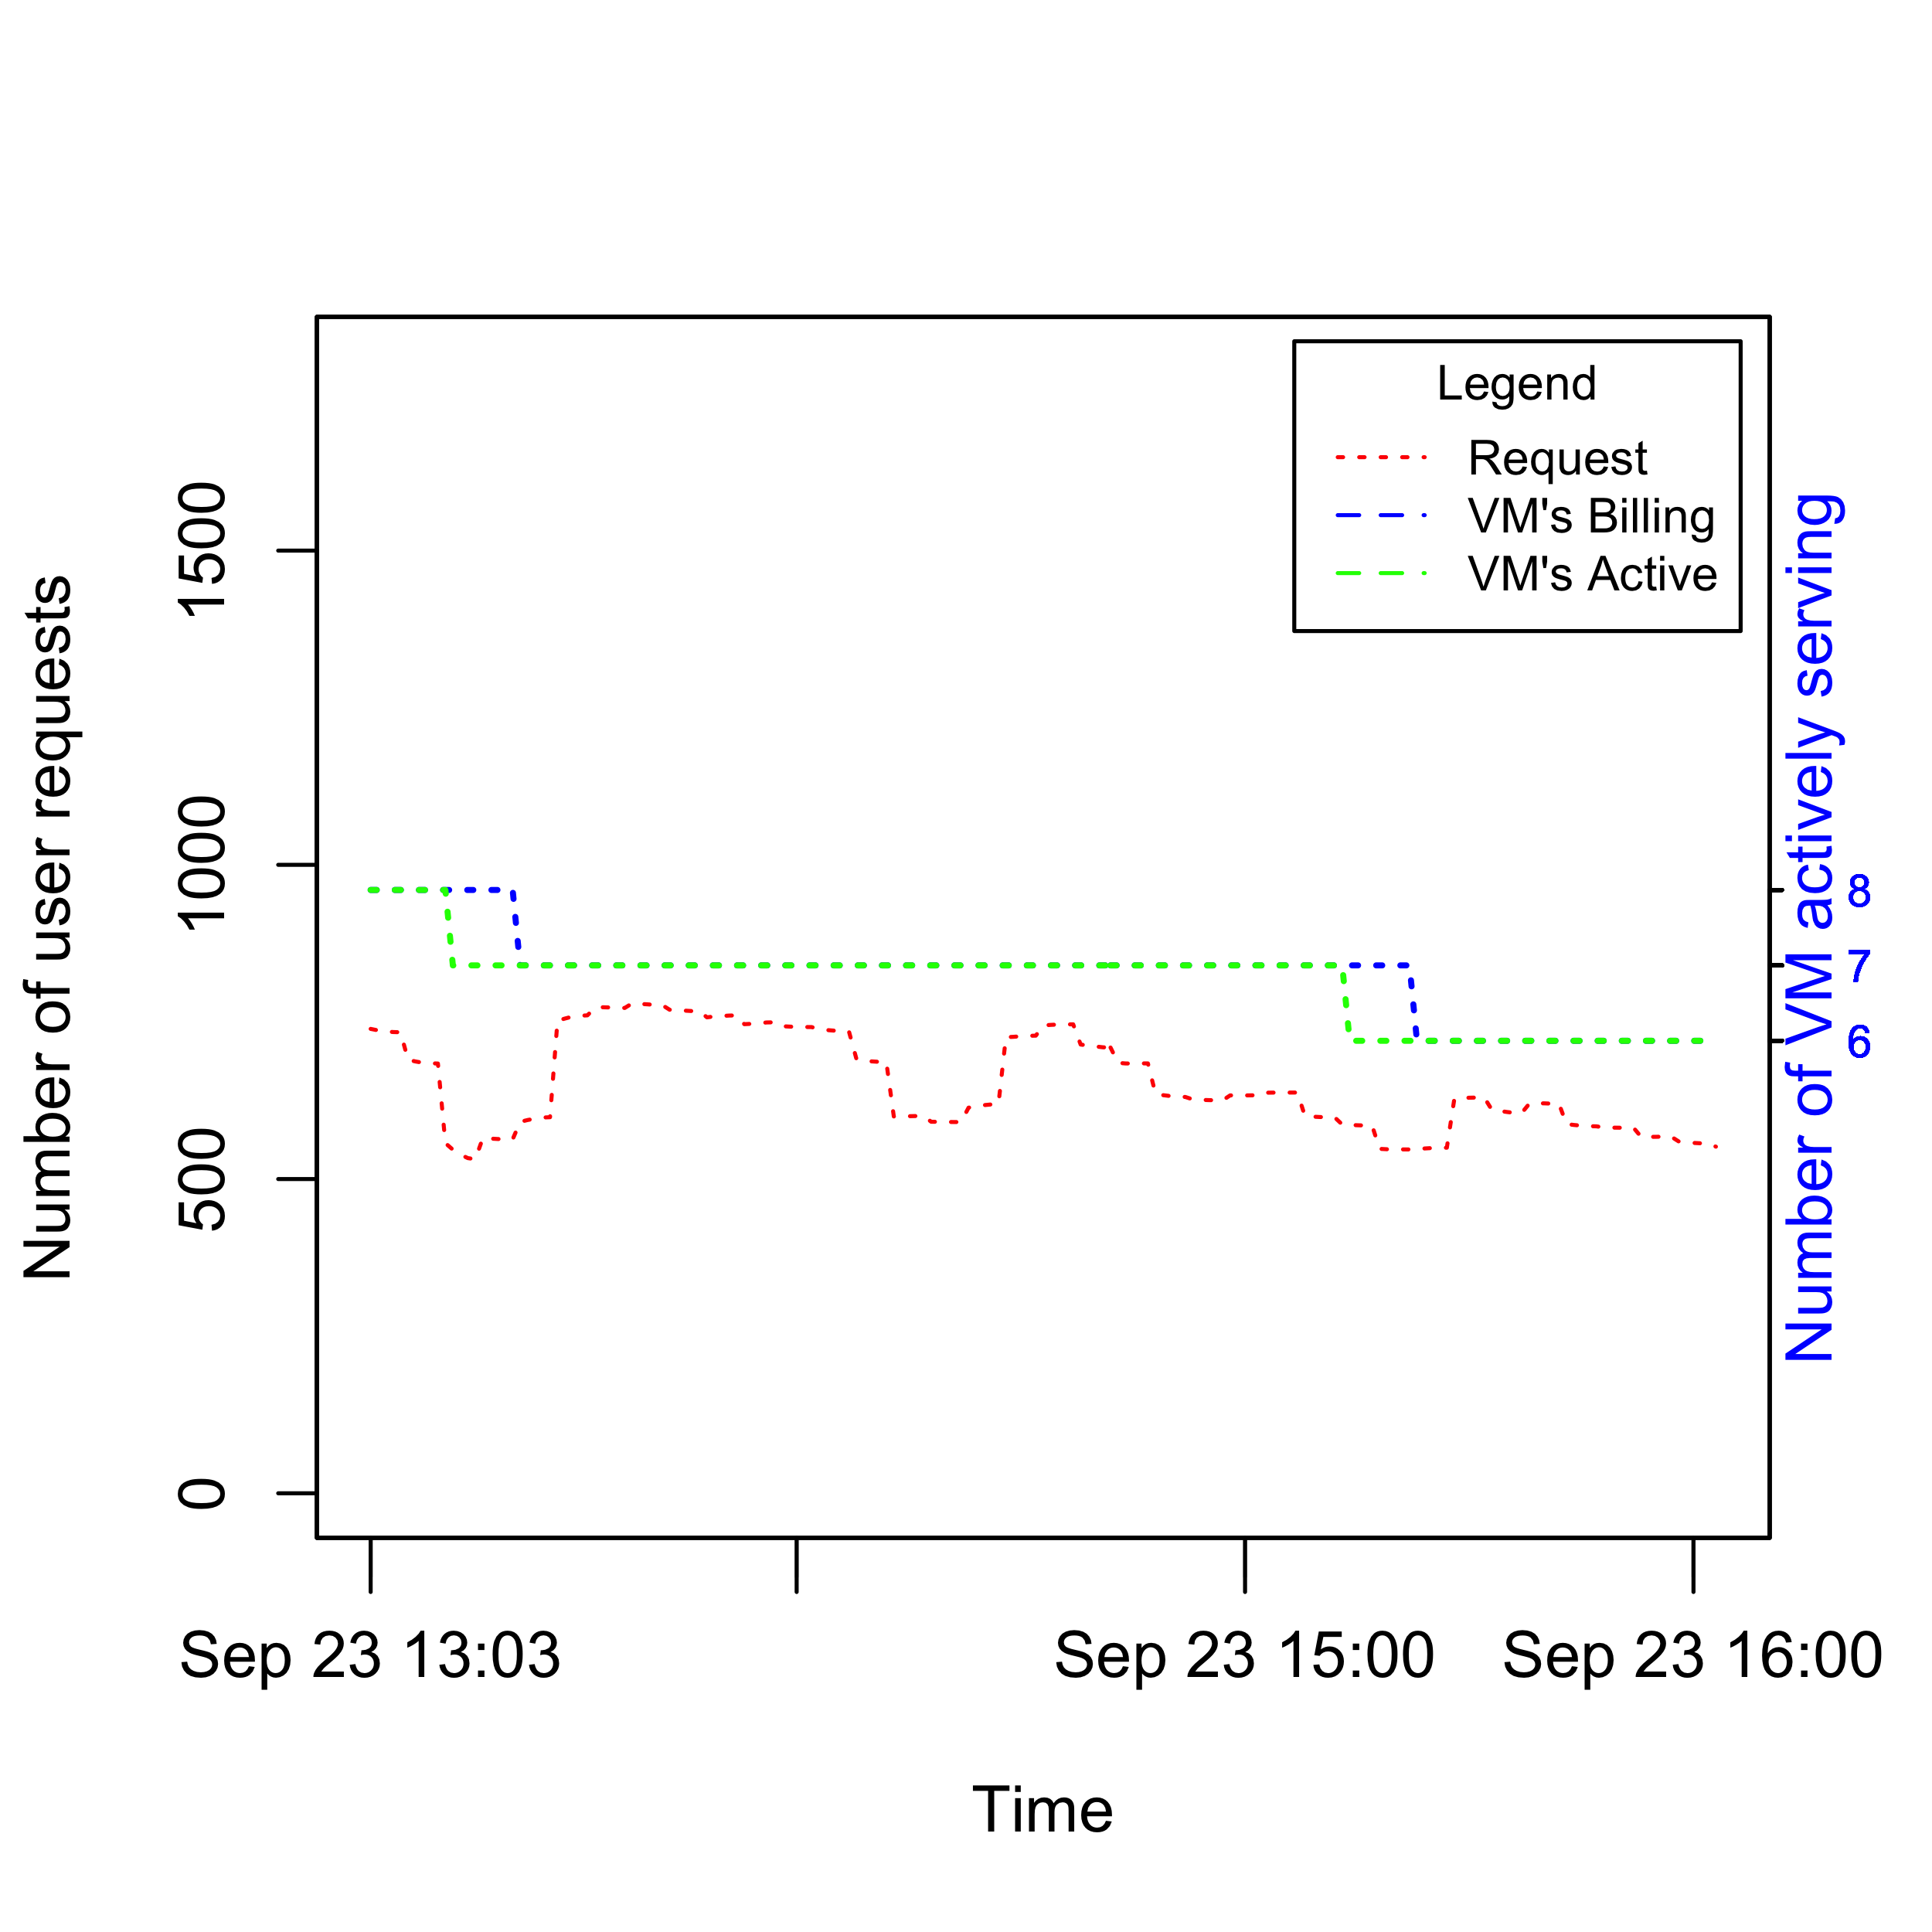
\includegraphics[width=\textwidth]{autoscalingdiag3.png}
         \caption{Decreasing in user request}
         \label{figure:autoscalingdiag3}
     \end{subfigure}
      \hfill
     \begin{subfigure}[b]{0.4\textwidth}
         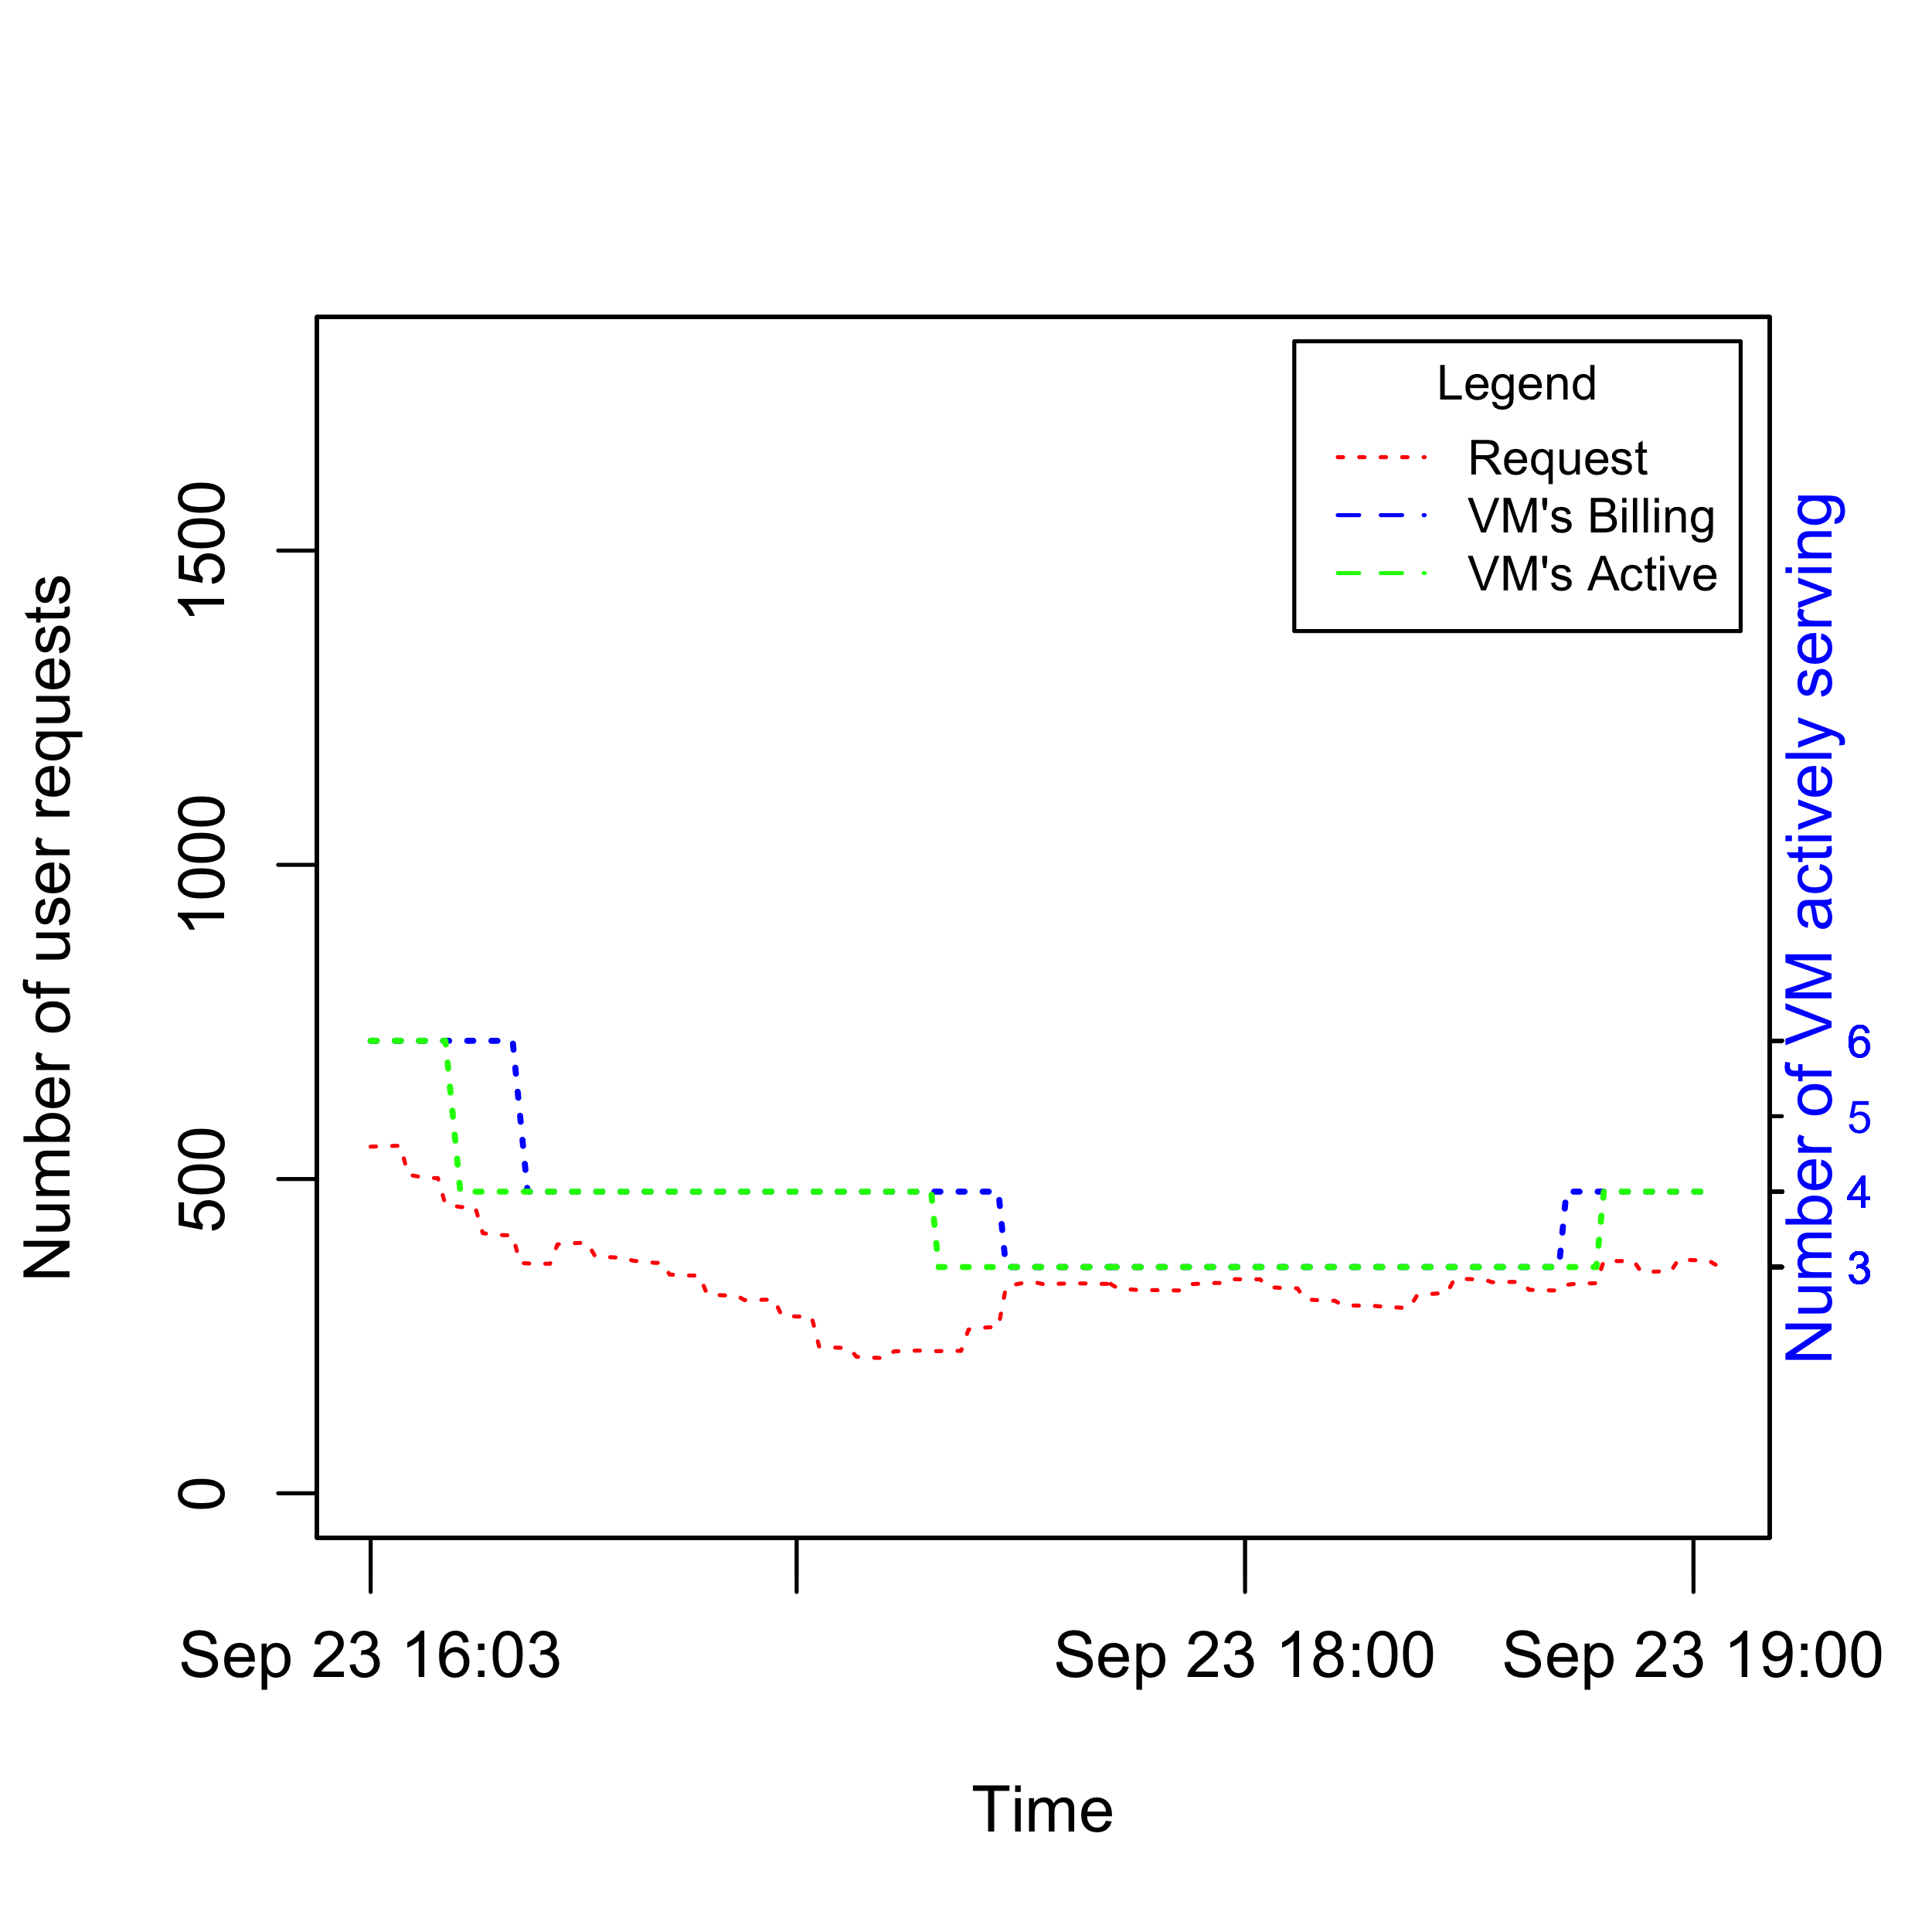
\includegraphics[width=\textwidth]{autoscalingdiag4.png}
         \caption{Decreasing in user request}
         \label{figure:autoscalingdiag4}
     \end{subfigure}
     \caption{AppElastic Performace on Workload}
     \label{fig:appelasticperformance}
 \end{figure}

\subsection{Forecast Accuracy}
\label{sub:Forecast Accuracy}
As discussed in the previous chapter, automated ARIMA model is used to forecast two type of data. These forecast data aids AppElastic for scale up lookahead and scale down lookahead features. Figure~\ref{fig:forecast} show the forecast plot of actual number of user request along with forecasted values. Based on the forecast horizon specified in ElasticSim configuration, forecasts are produced for scale up in Figure~\ref{figure:forecastscaleup} and for scale down as shown in Figure~\ref{figure:forecastscaledown}. As introduced in section~\ref{sec:implementationprediction} percentage error is used to measured the accuracy. MAPE Percentage errors have the advantage of being scale-independent, and frequently used to compare forecast performance between different data sets. Box plot of forecast errors are as shown in Figure~\ref{fig:forecasterror}. Using automated ARIMA modeling building with R \(auto.arima()\) function has produced forecast with mean error of 1.5\% in both scale up and scale down forecasts.
\begin{figure}
     \centering
     \begin{subfigure}[b]{0.9\textwidth}
         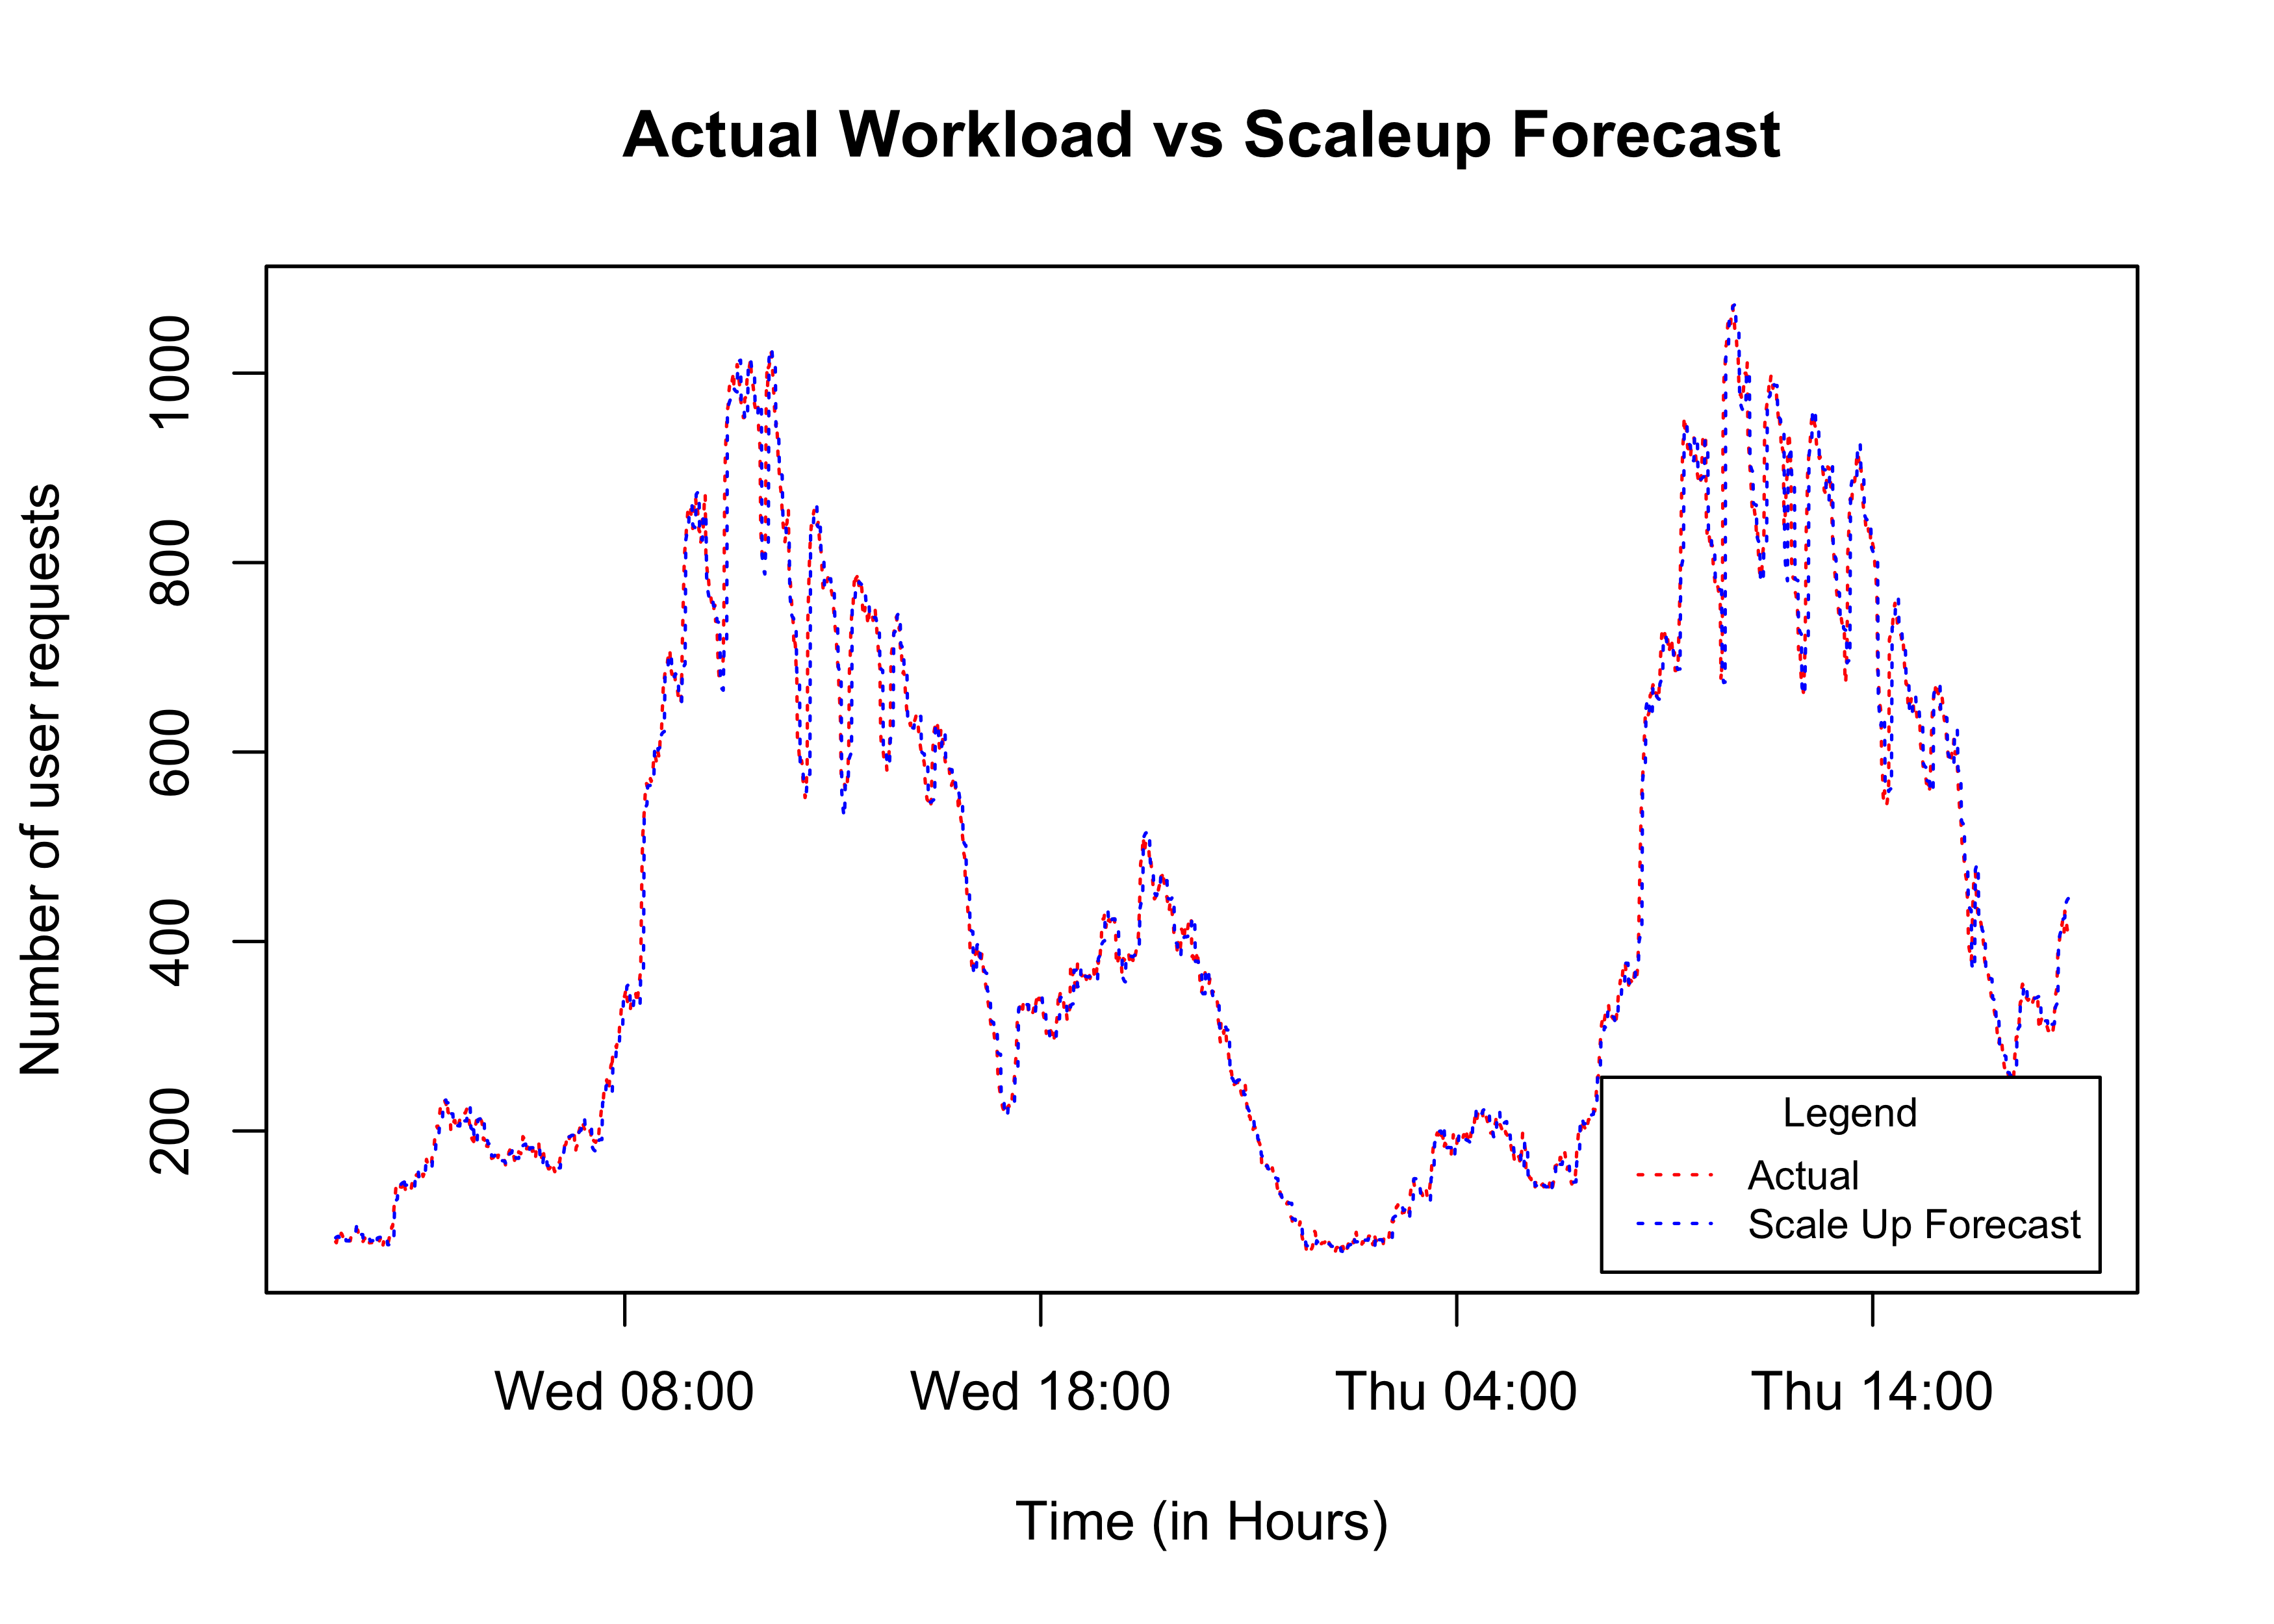
\includegraphics[width=\textwidth]{ScaleUpForecast.png}
         \caption{Scale up forecast}
         \label{figure:forecastscaleup}
     \end{subfigure}
     \begin{subfigure}[b]{0.9\textwidth}
         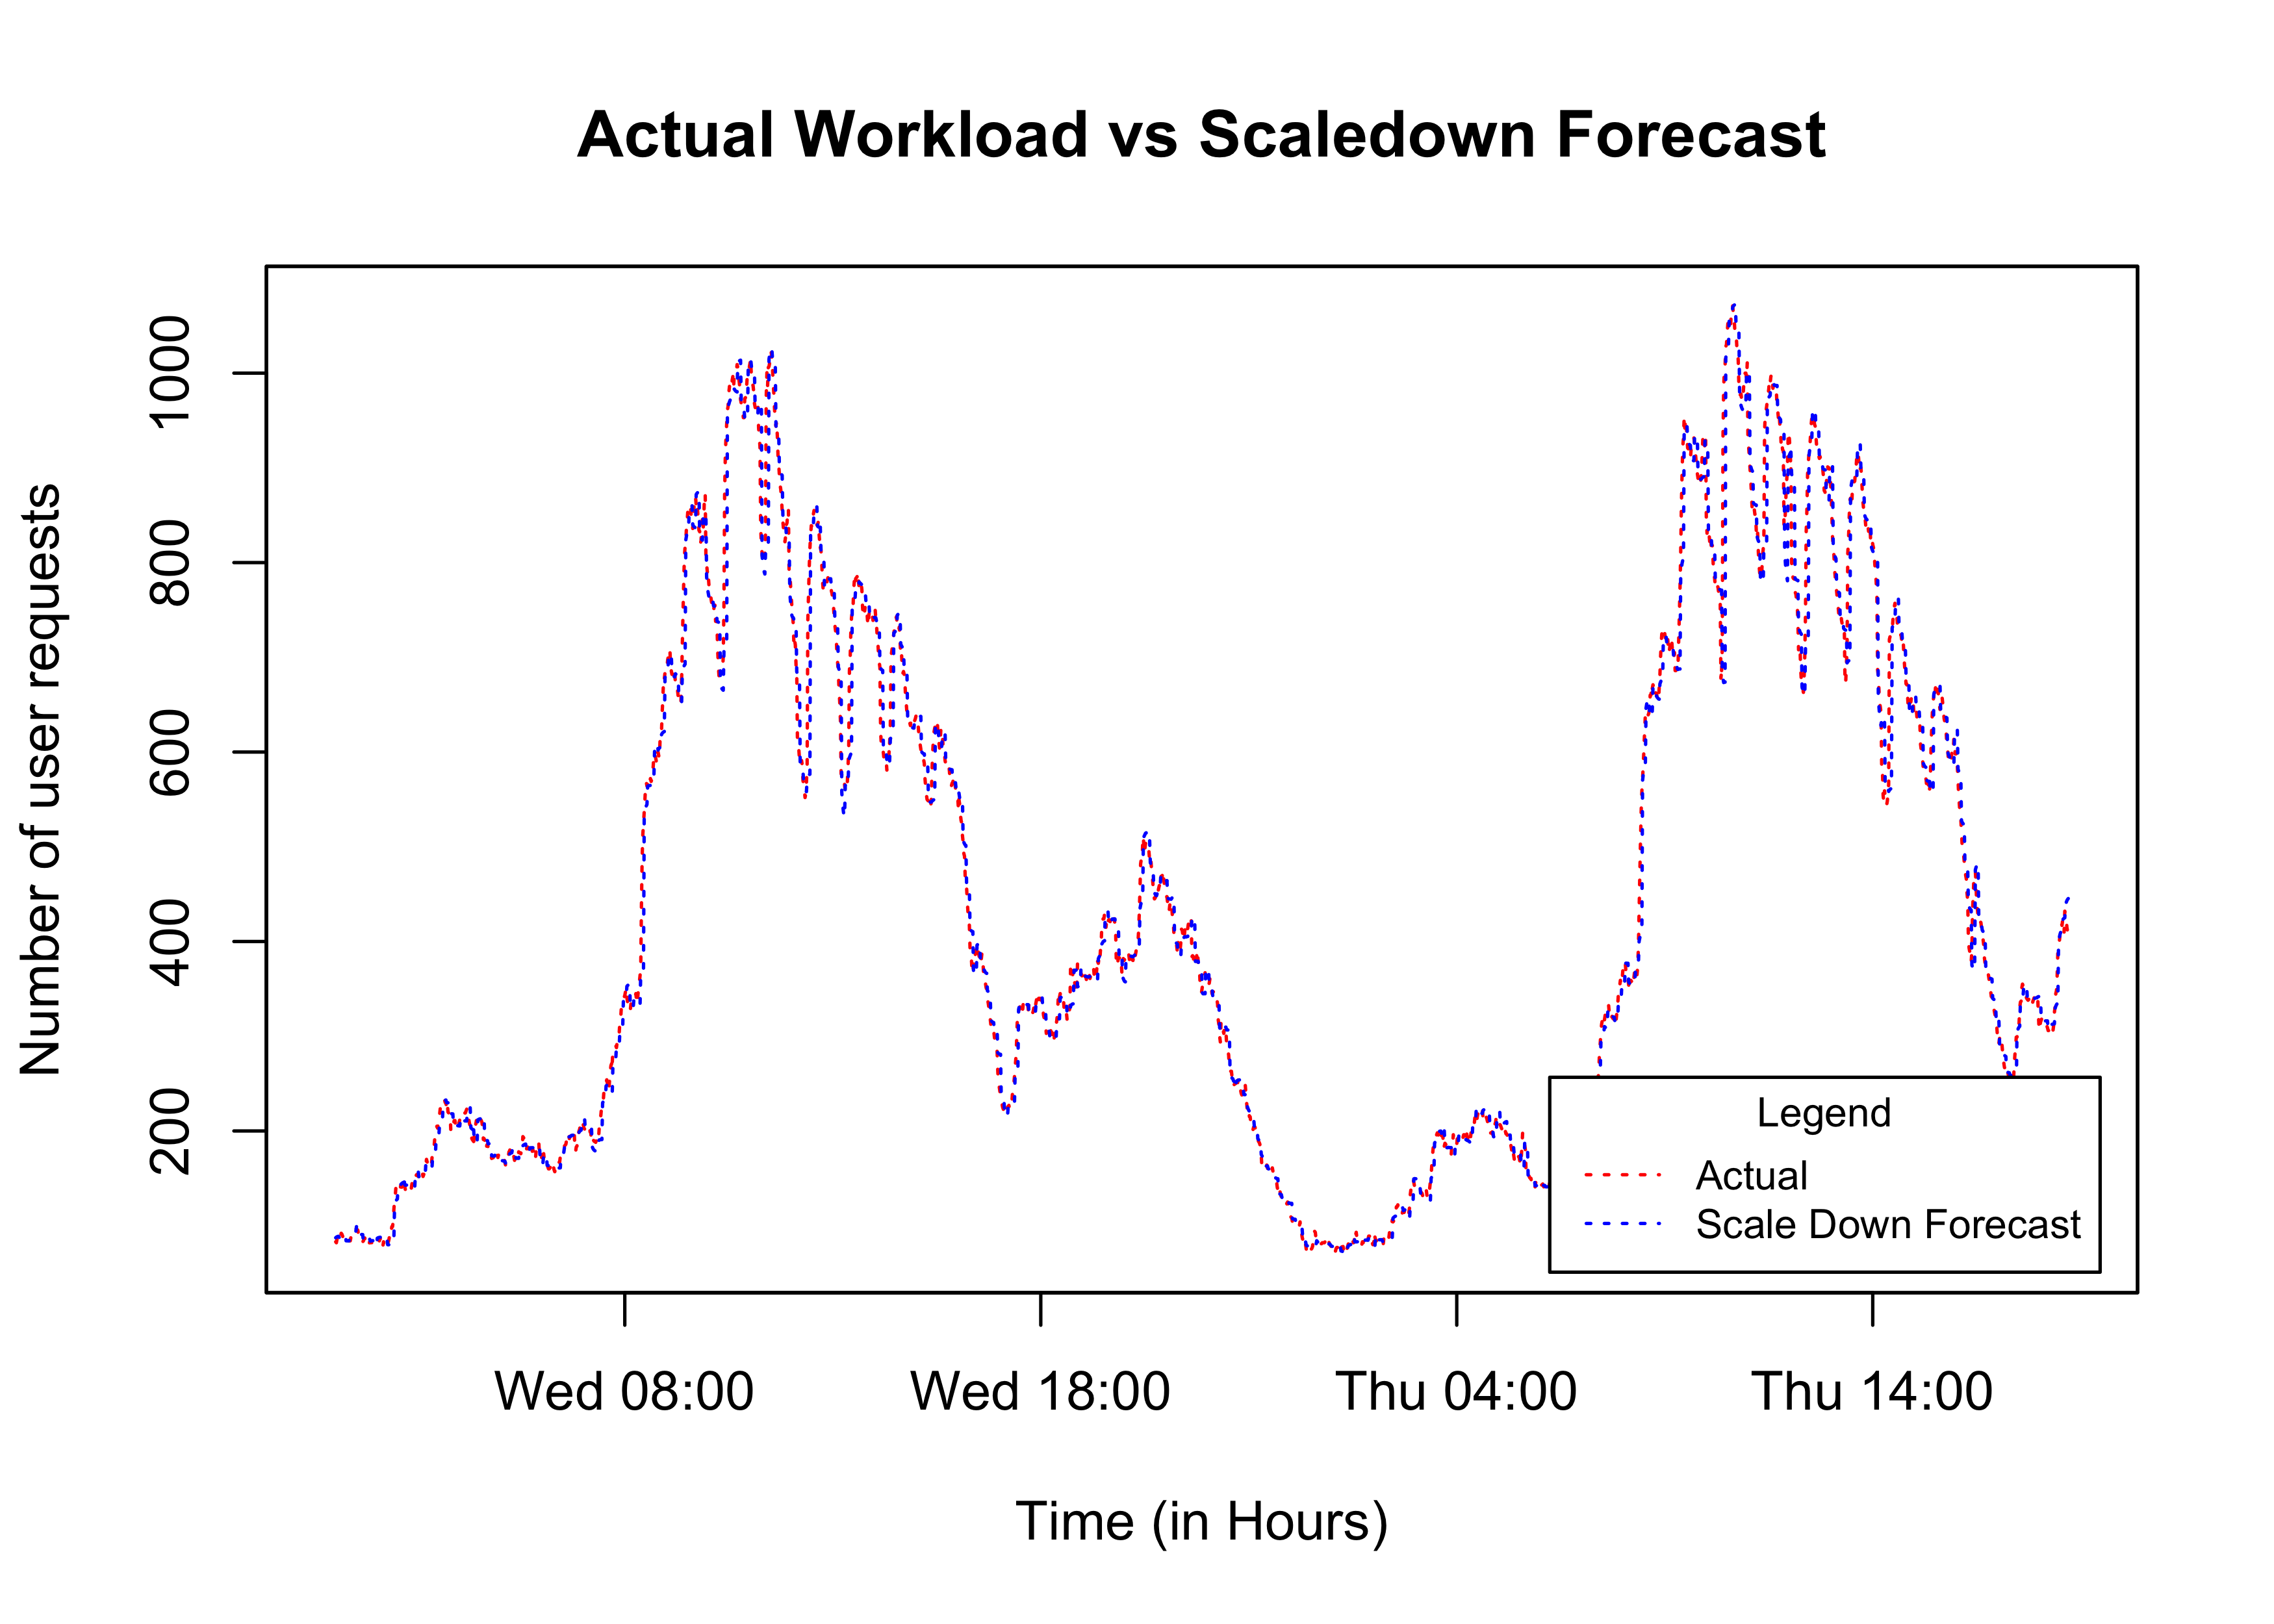
\includegraphics[width=\textwidth]{ScaleDownForecast.png}
         \caption{Scale down forecast}
         \label{figure:forecastscaledown}
     \end{subfigure}
     \caption{Forecast for Scale Up and Down}
     \label{fig:forecast}
\end{figure}
\begin{figure}
     \centering
     \begin{subfigure}[b]{0.45\textwidth}
         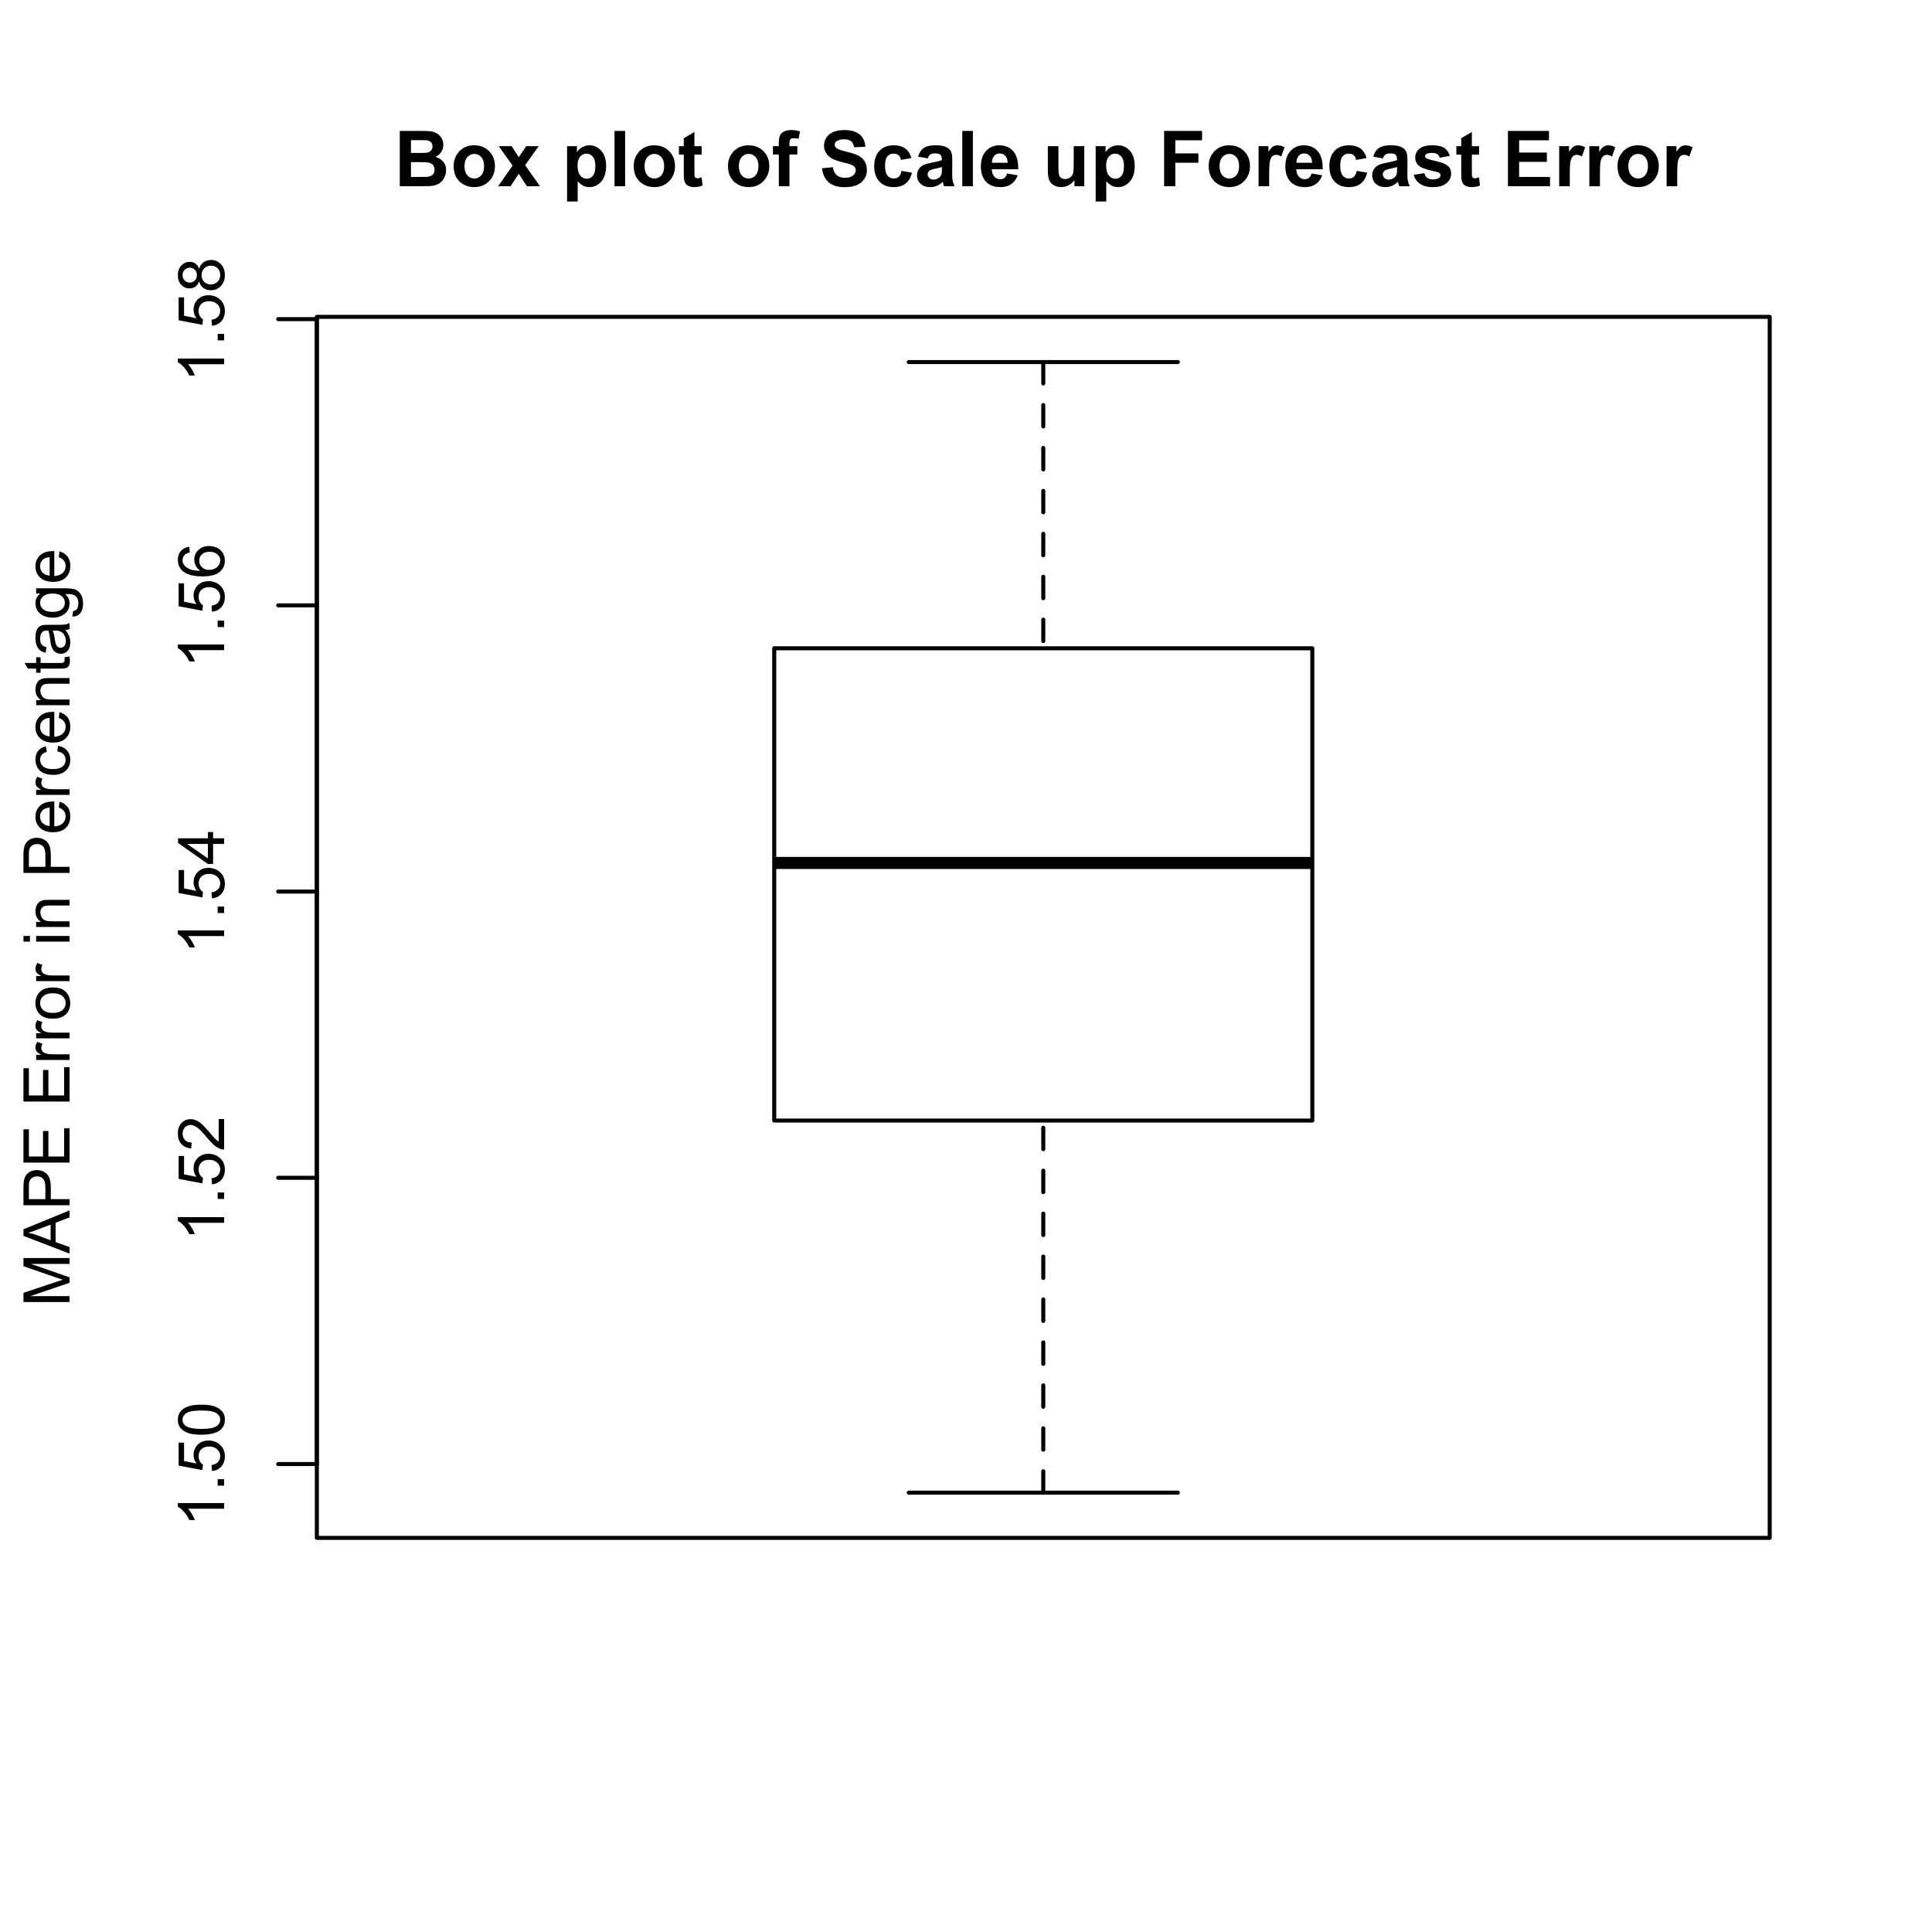
\includegraphics[width=\textwidth]{ScaleUpAcc.png}
         \caption{Scale up forecast error}
         \label{figure:forecastscaleuperror}
     \end{subfigure}
     \hfill
     \begin{subfigure}[b]{0.45\textwidth}
         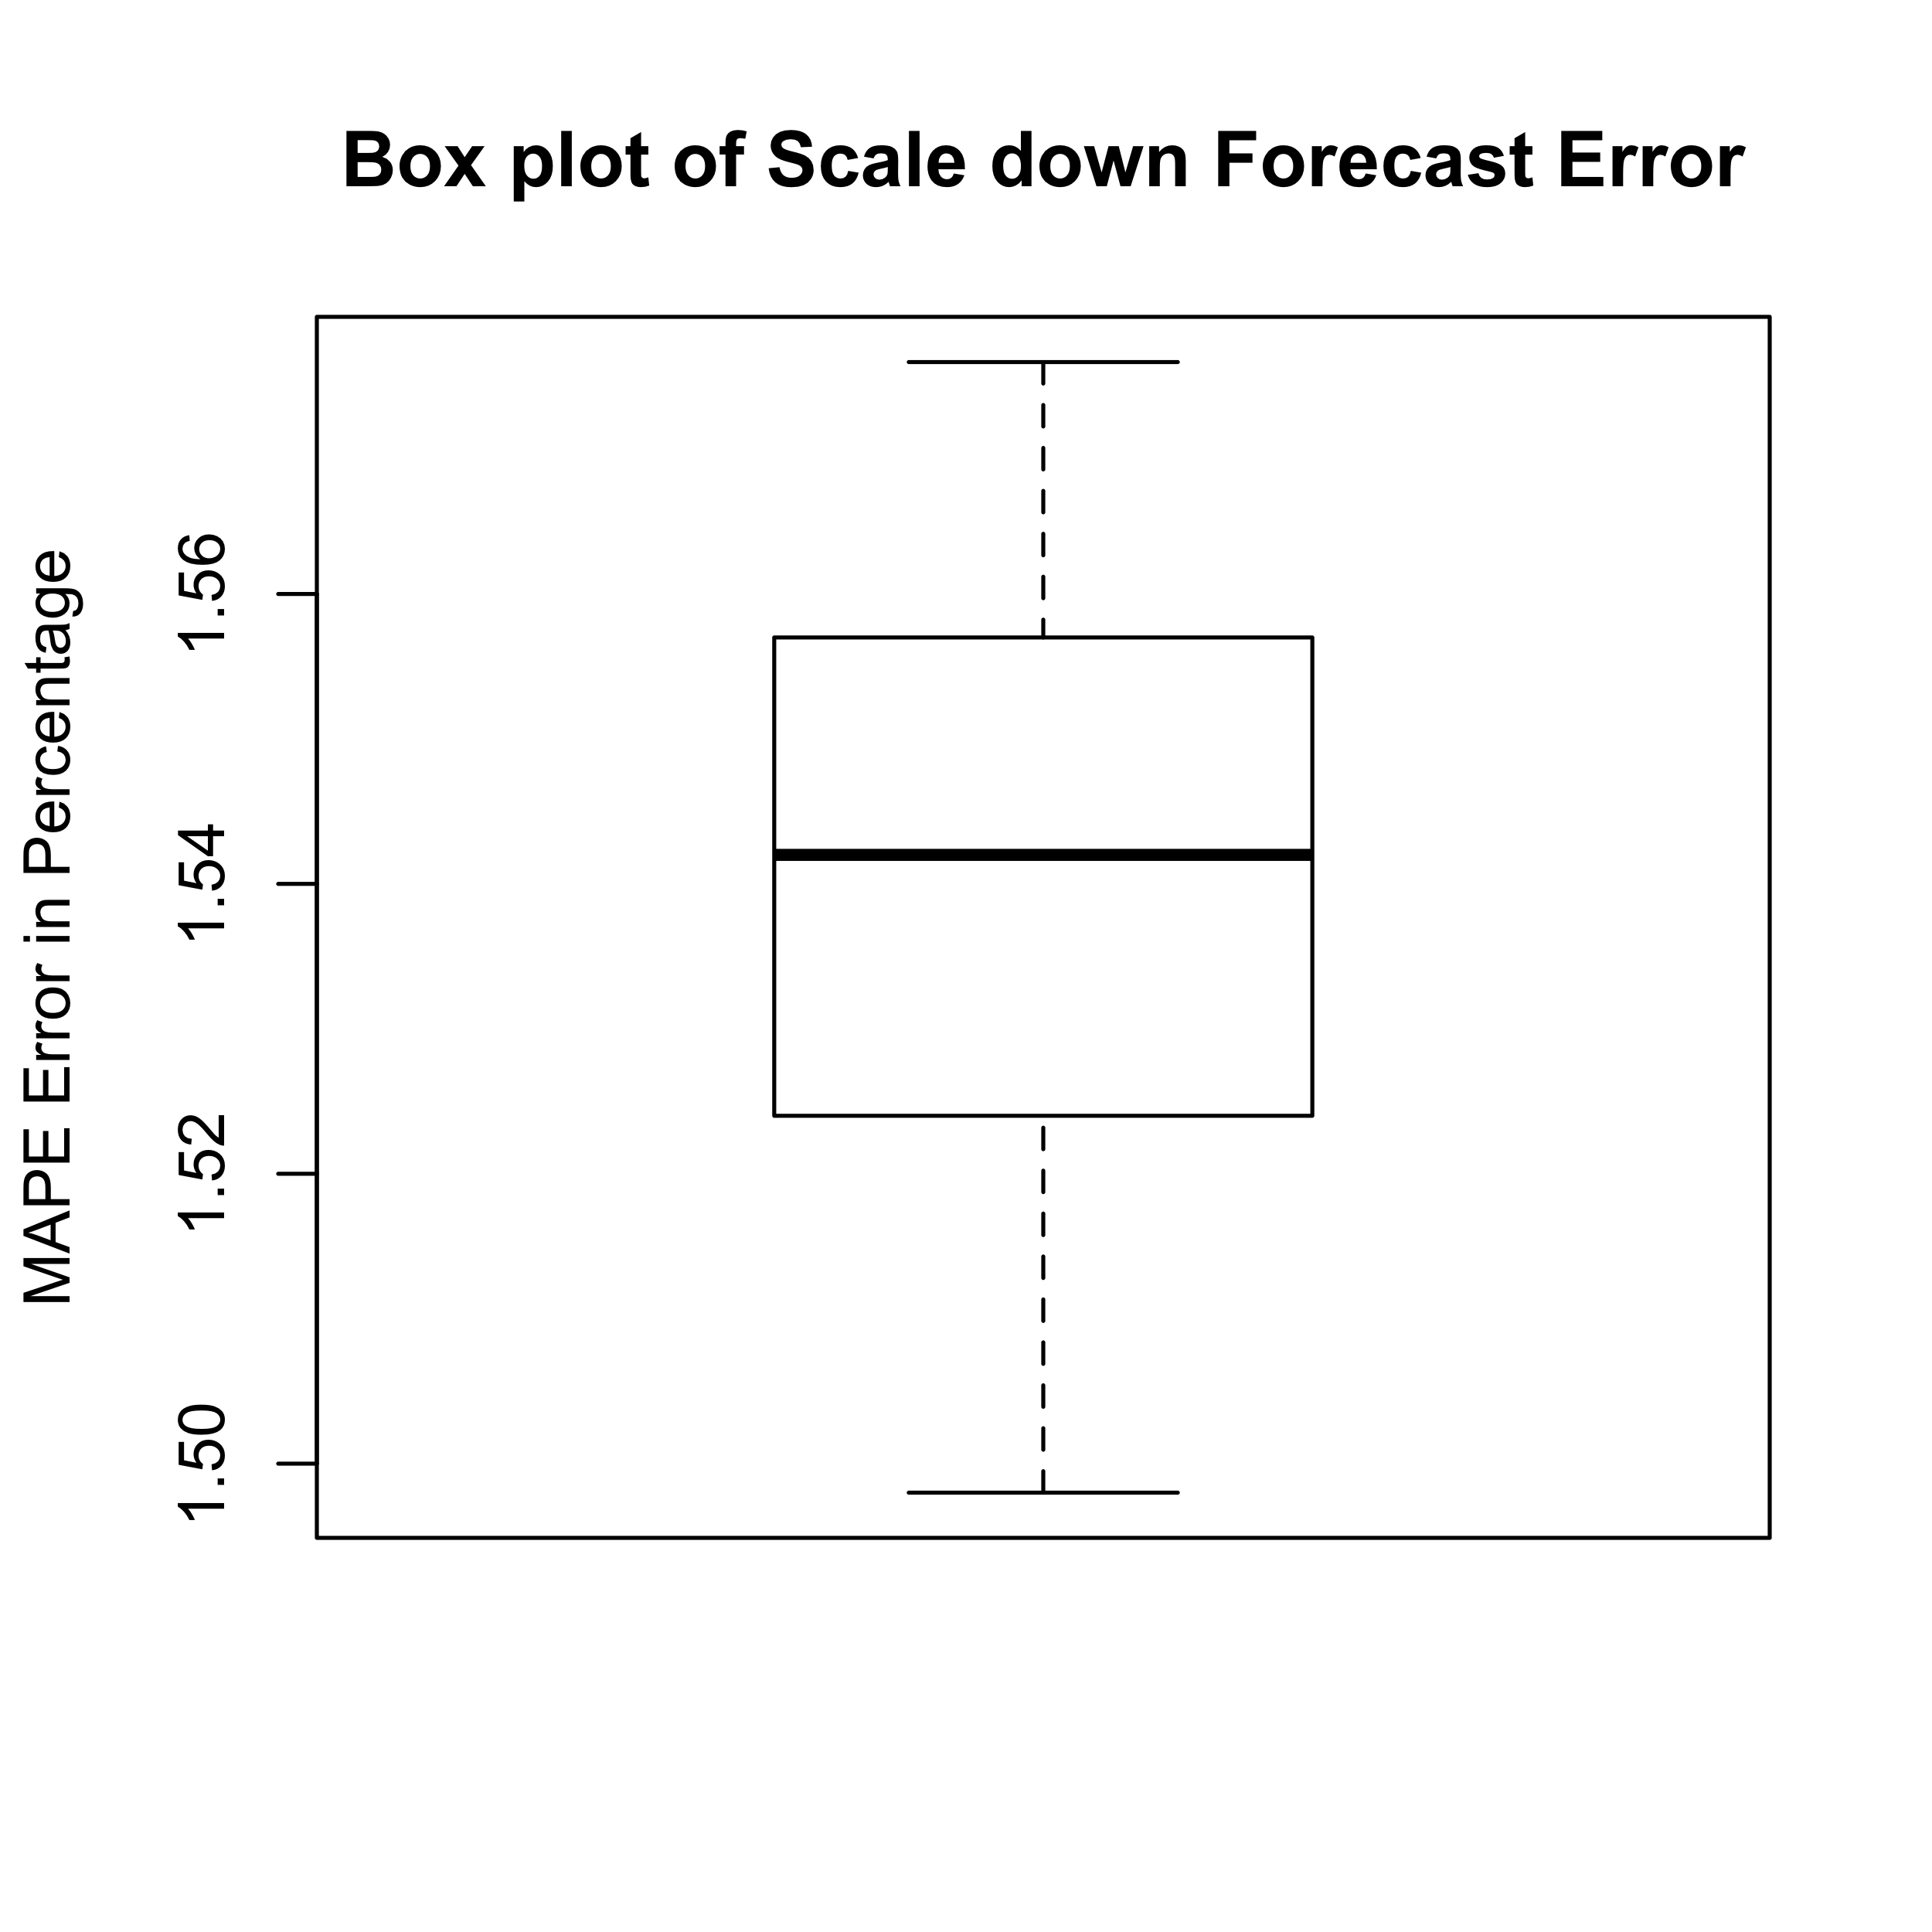
\includegraphics[width=\textwidth]{ScaleDownAcc.png}
         \caption{Scale down forecast error}
         \label{figure:forecastscaledownerror}
     \end{subfigure}
     \caption{Forecast Errors}
     \label{fig:forecasterror}
\end{figure}
\subsection{SLA violation}
\label{sub:SLA violation}
As discussed in section~\ref{subs:AppElastic with Look-ahead}, AppElastic algorithm will run on the predicted workloads which is generated by ARIMA model. As it was clear form the previous section, ARIMA model has forecast error of 1.5\% in both scale up and scale down forecasts. These forecast error leads to SLA violations\footnote{Refer section~\ref{sec:SLA Violations}}. Figure~\ref{fig:forecasterror} some examples of SLA violation due to forecast error. As its shown in the figure, number of VM active will not be enough to server the user request. Equation~\ref{eq:userslavio} is used to calculate how many of these user SLA violation and have degraded quality of services or no service. As show in the case analysis~\ref{eq:slaviocase}, SLA violation will occur when the required number of VM's to fulfill user reqest is more than number of VM's active. These SLA violation is evident from the experiments conducted and the graphs related to these SLA violations are in Figure~\ref{fig:slaviolationgraphs}. As its show in the Figure~\ref{figure:slaviolation1} and Figure~\ref{figure:slaviolation2}, number of VM's active in some parts of the graph are less than the number of user request arriving to the system. Figure~\ref{figure:boxplotslaviolation} the boxplot of number of users for which SLA is violated. Based on the experiments up to 168 users has faced SLA violation.
\begin{equation}
\textrm{ Identify SLA Violations }=
  \begin{cases}
    VM_{required} - VM_{active} < 0 \textrm{ No SLA violation}\\
    VM_{required} - VM_{active} = 0 \textrm{ No SLA violation}\\
    VM_{required} - VM_{active} > 1 \textrm{ SLA violation}\\
\end{cases}
\label{eq:slaviocase}
\end{equation}
\begin{equation}
Users_{\textrm{SLA violation}} = UserRequest_{t} - Capaticy_{t}
\label{eq:userslavio}
\end{equation}
\begin{figure}
     \centering
     \begin{subfigure}[b]{0.45\textwidth}
         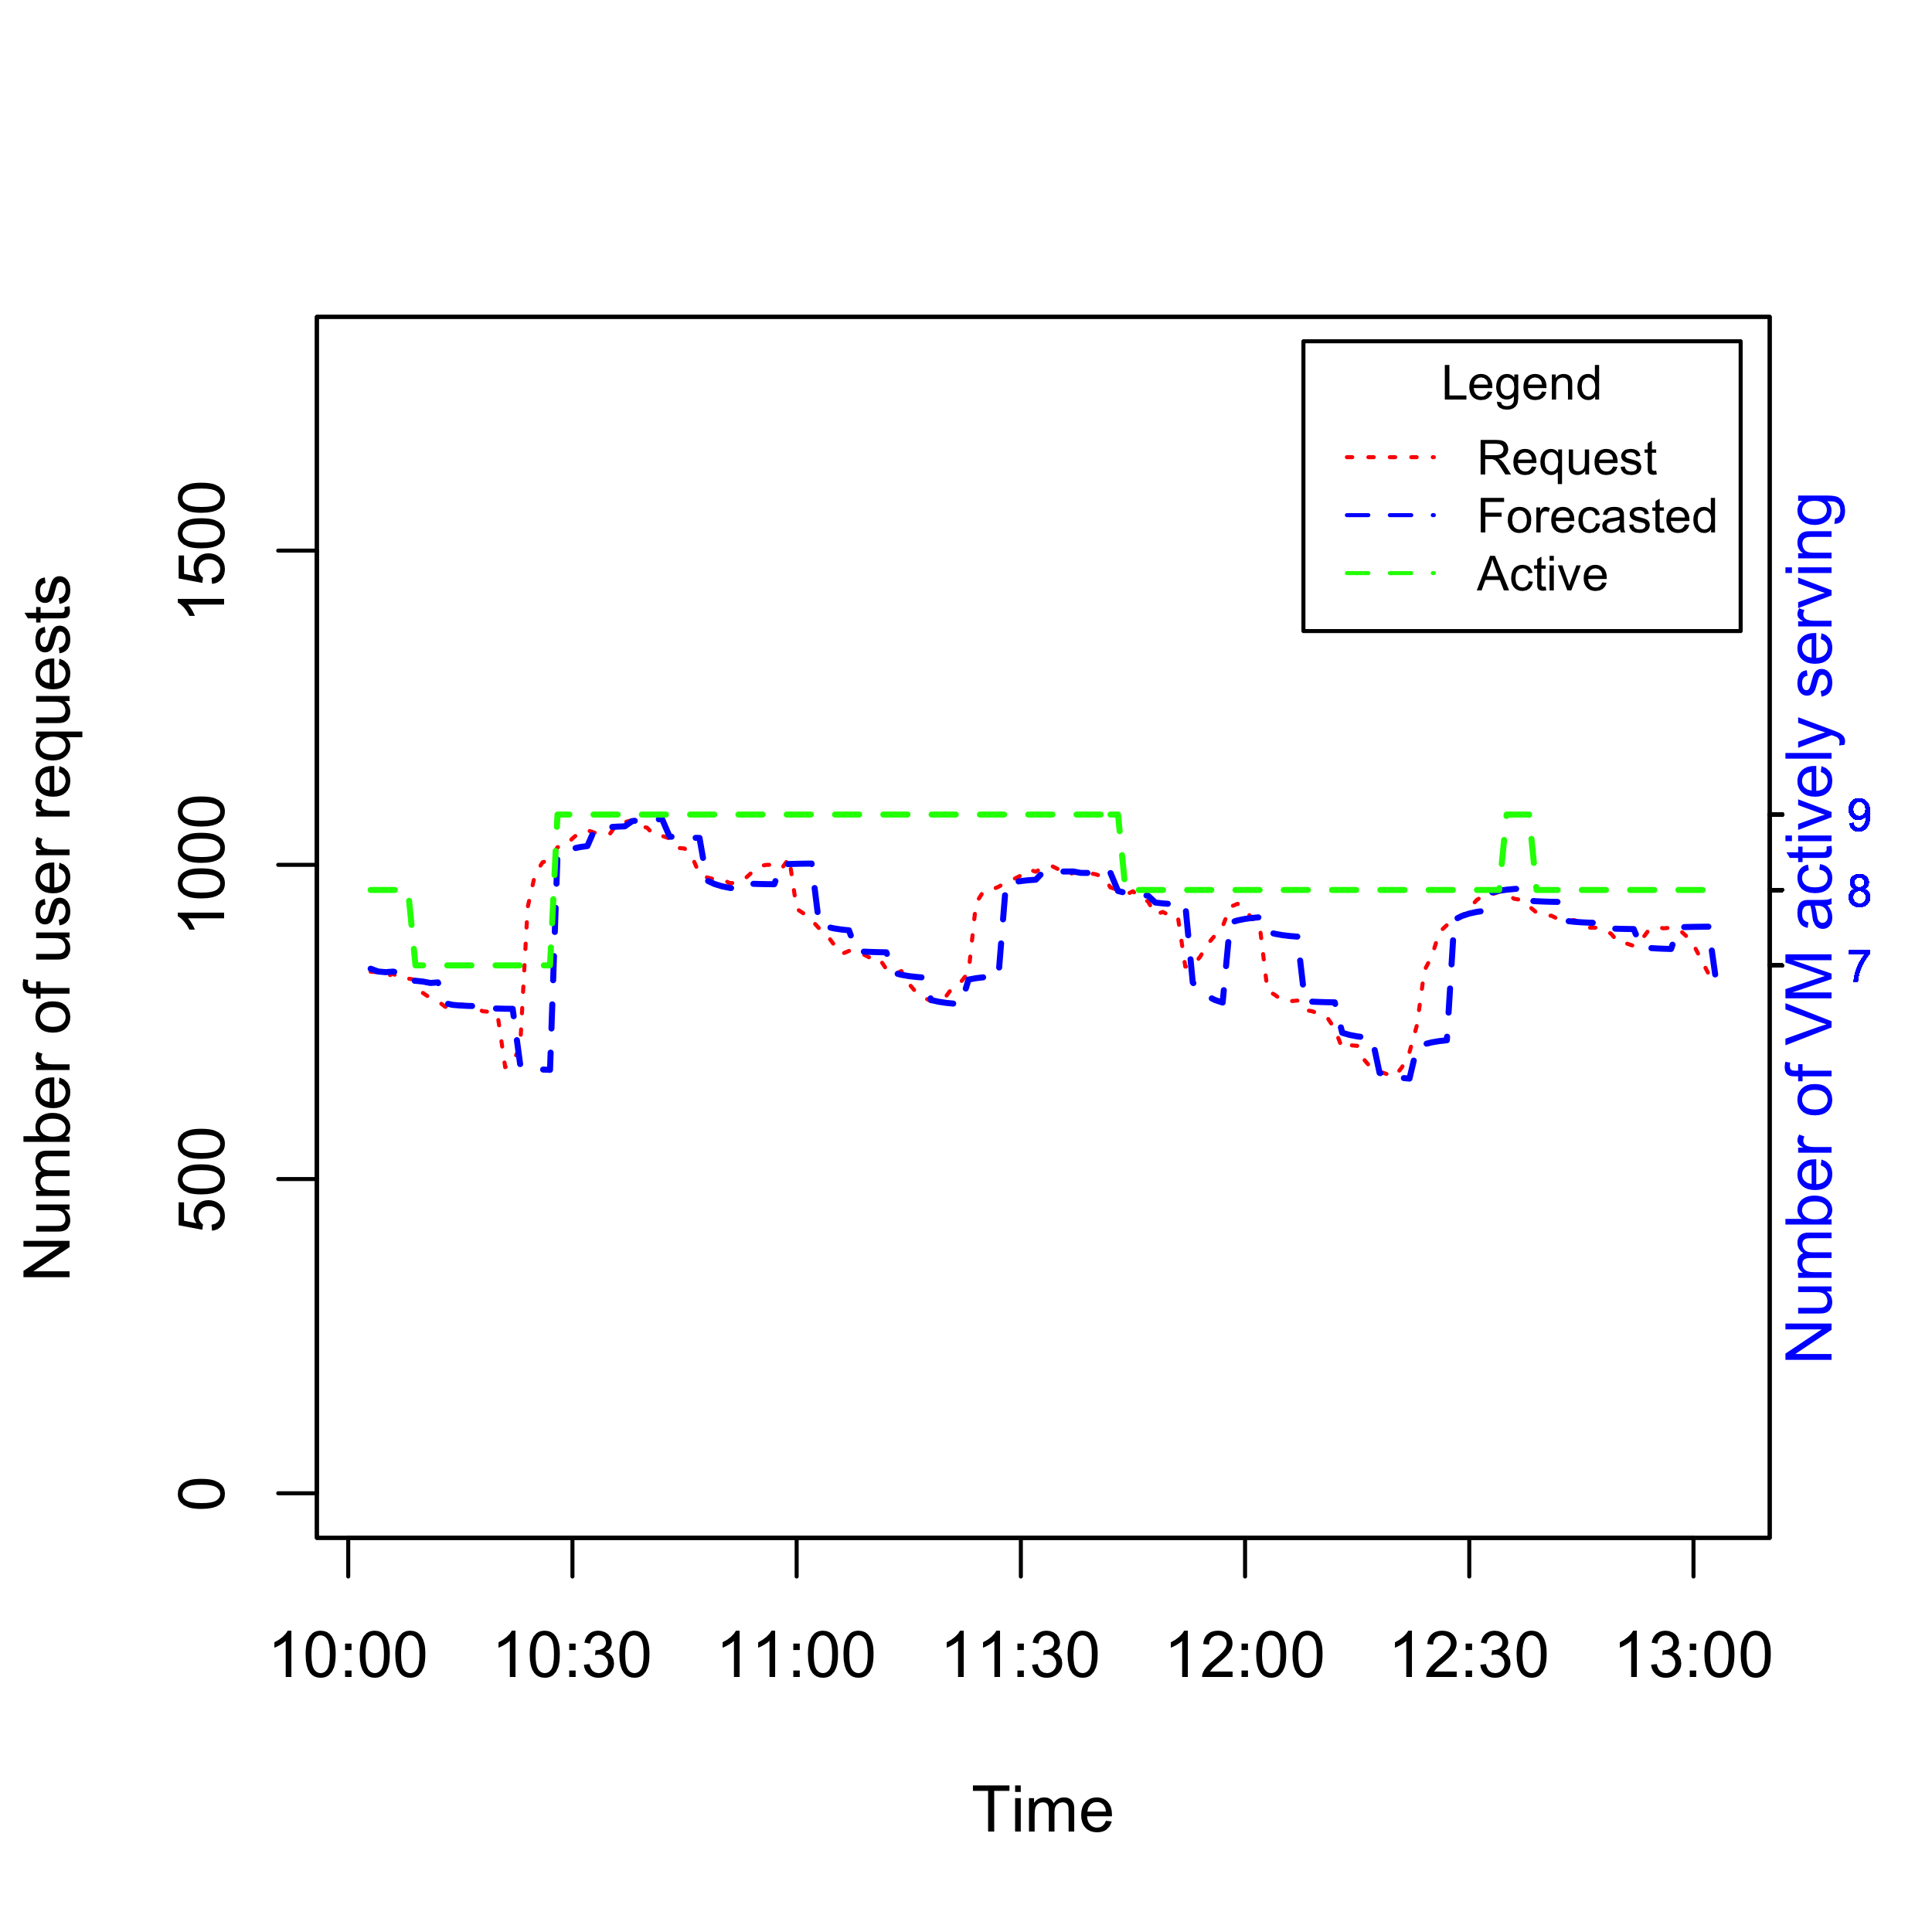
\includegraphics[width=\textwidth]{slaviolation1.png}
         \caption{Example of SLA violation-1}
         \label{figure:slaviolation1}
     \end{subfigure}
     \hfill
     \begin{subfigure}[b]{0.45\textwidth}
         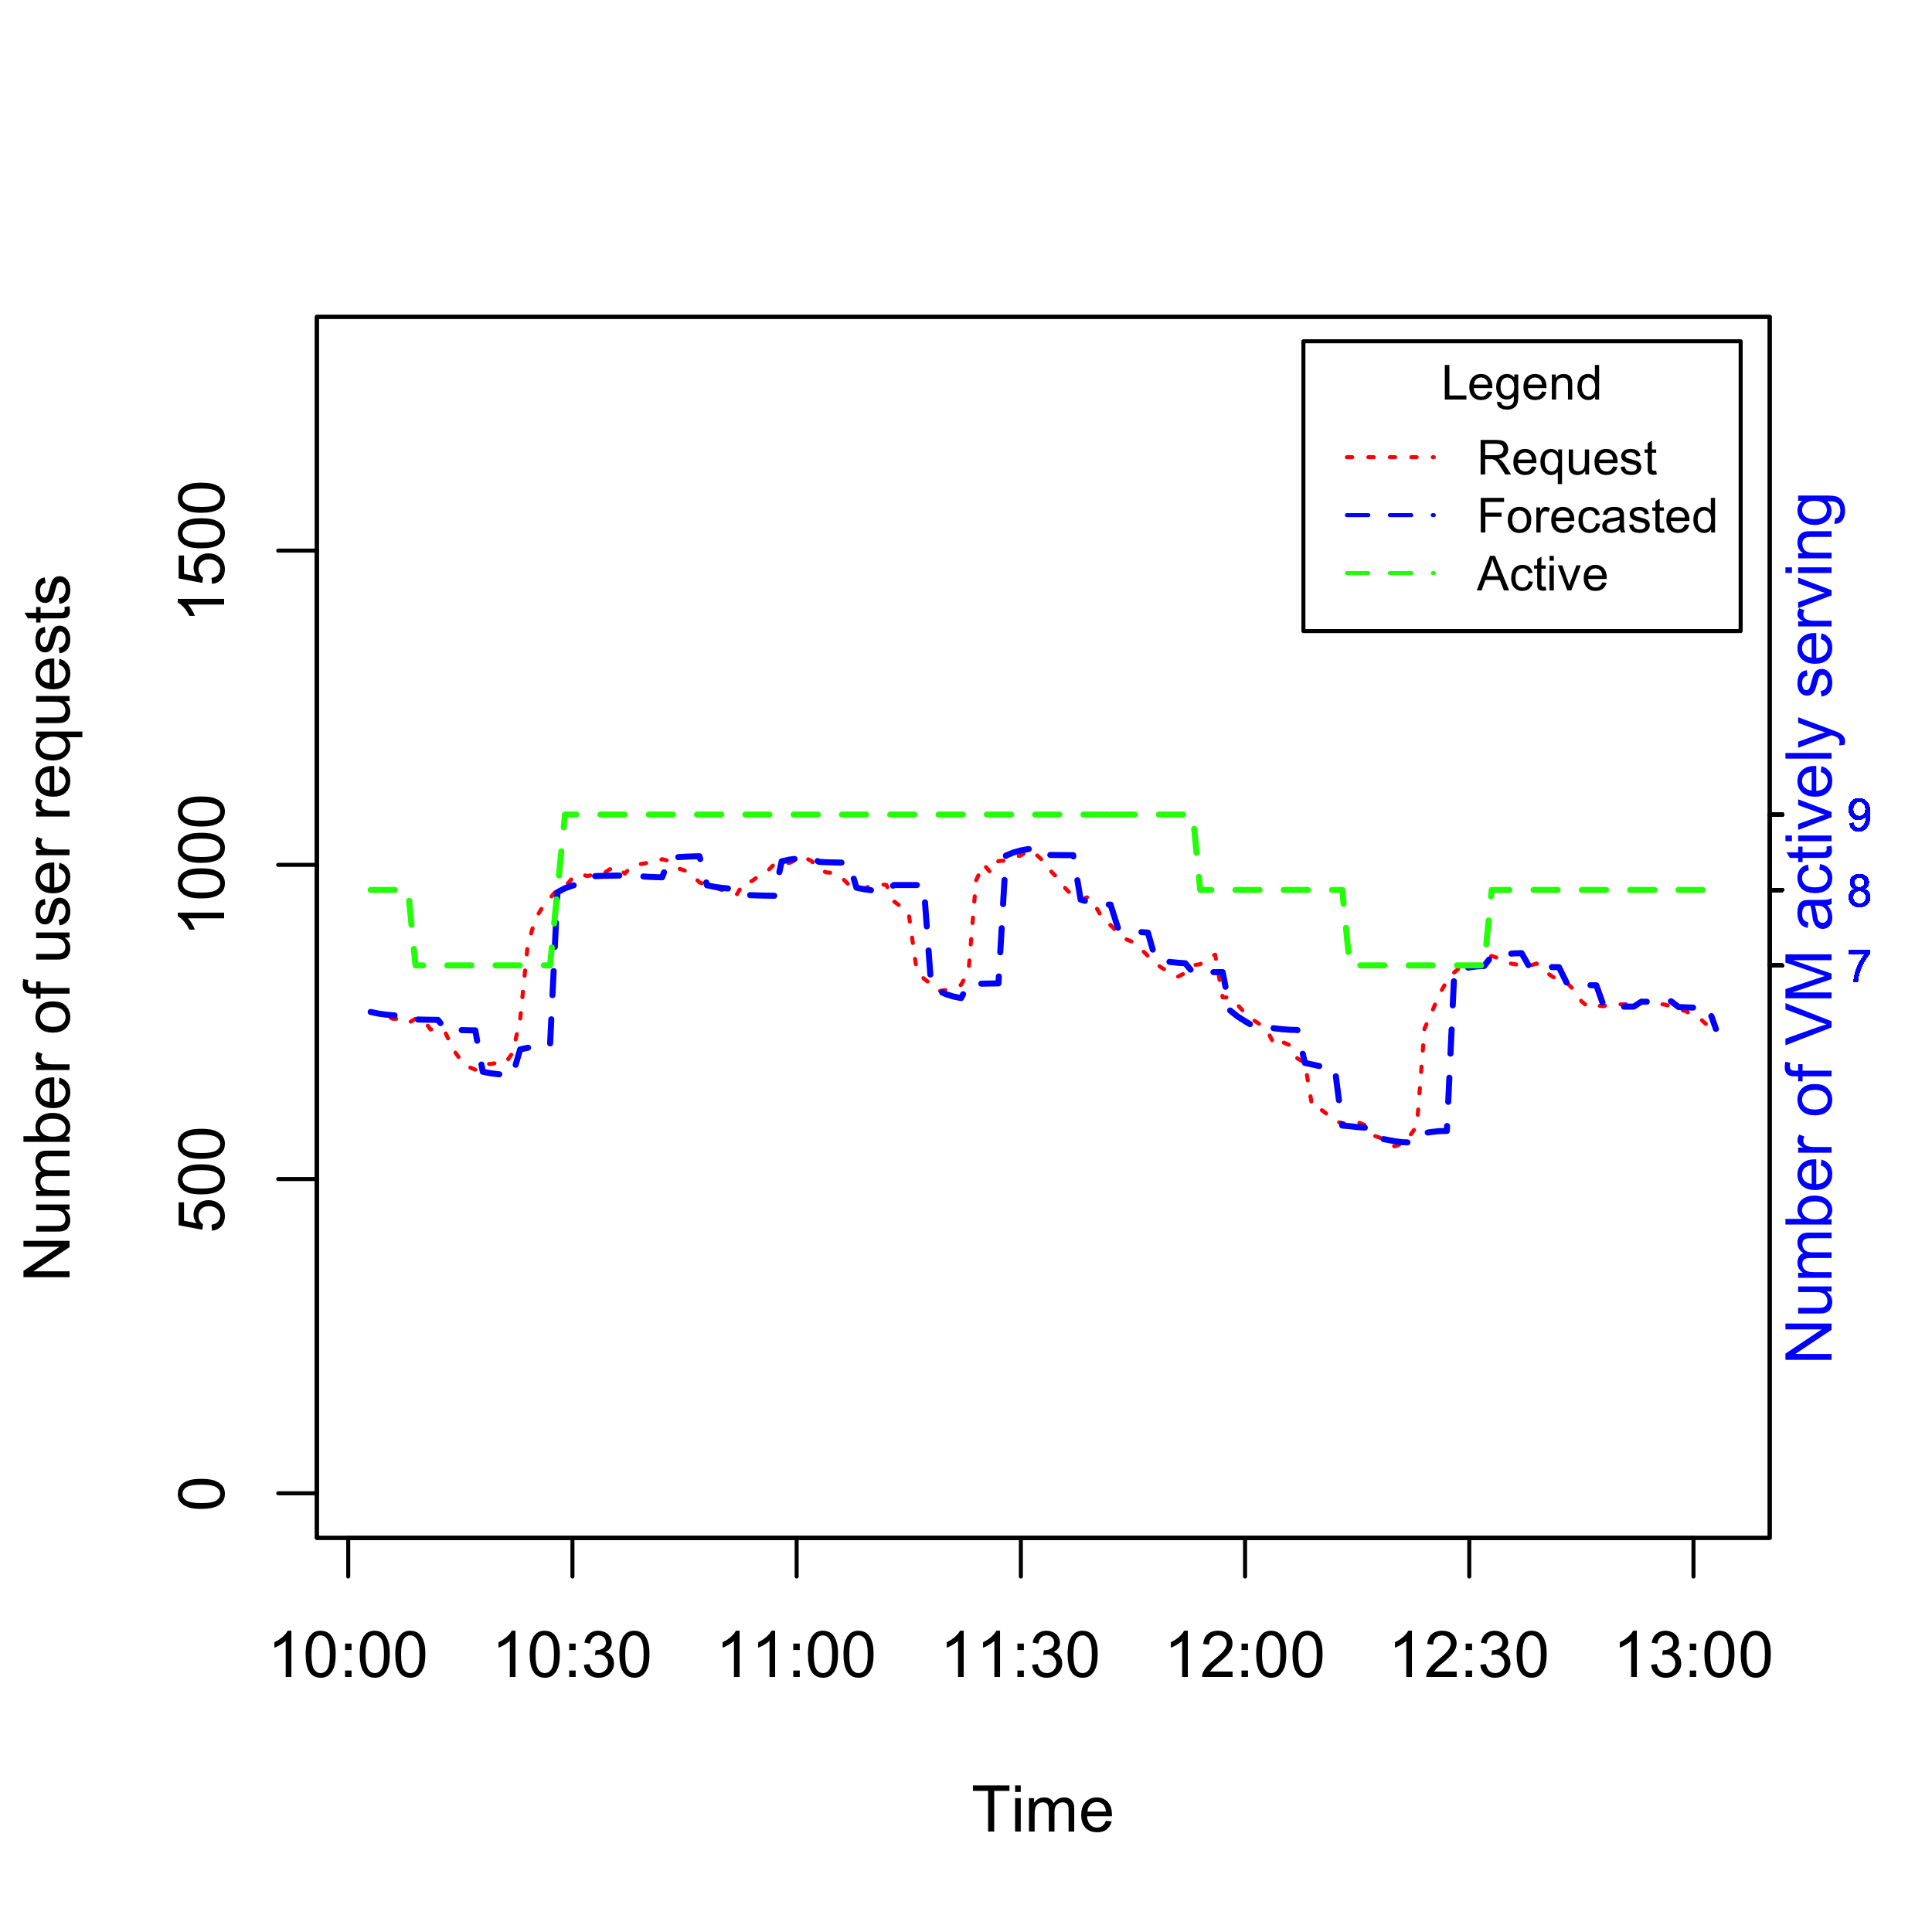
\includegraphics[width=\textwidth]{slaviolation2.png}
         \caption{Example of SLA violation-2}
         \label{figure:slaviolation2}
     \end{subfigure}
     \caption{SLA violation}
     \label{fig:slaviolationgraphs}
\end{figure}

\begin{figure}[h]
  \begin{center}
    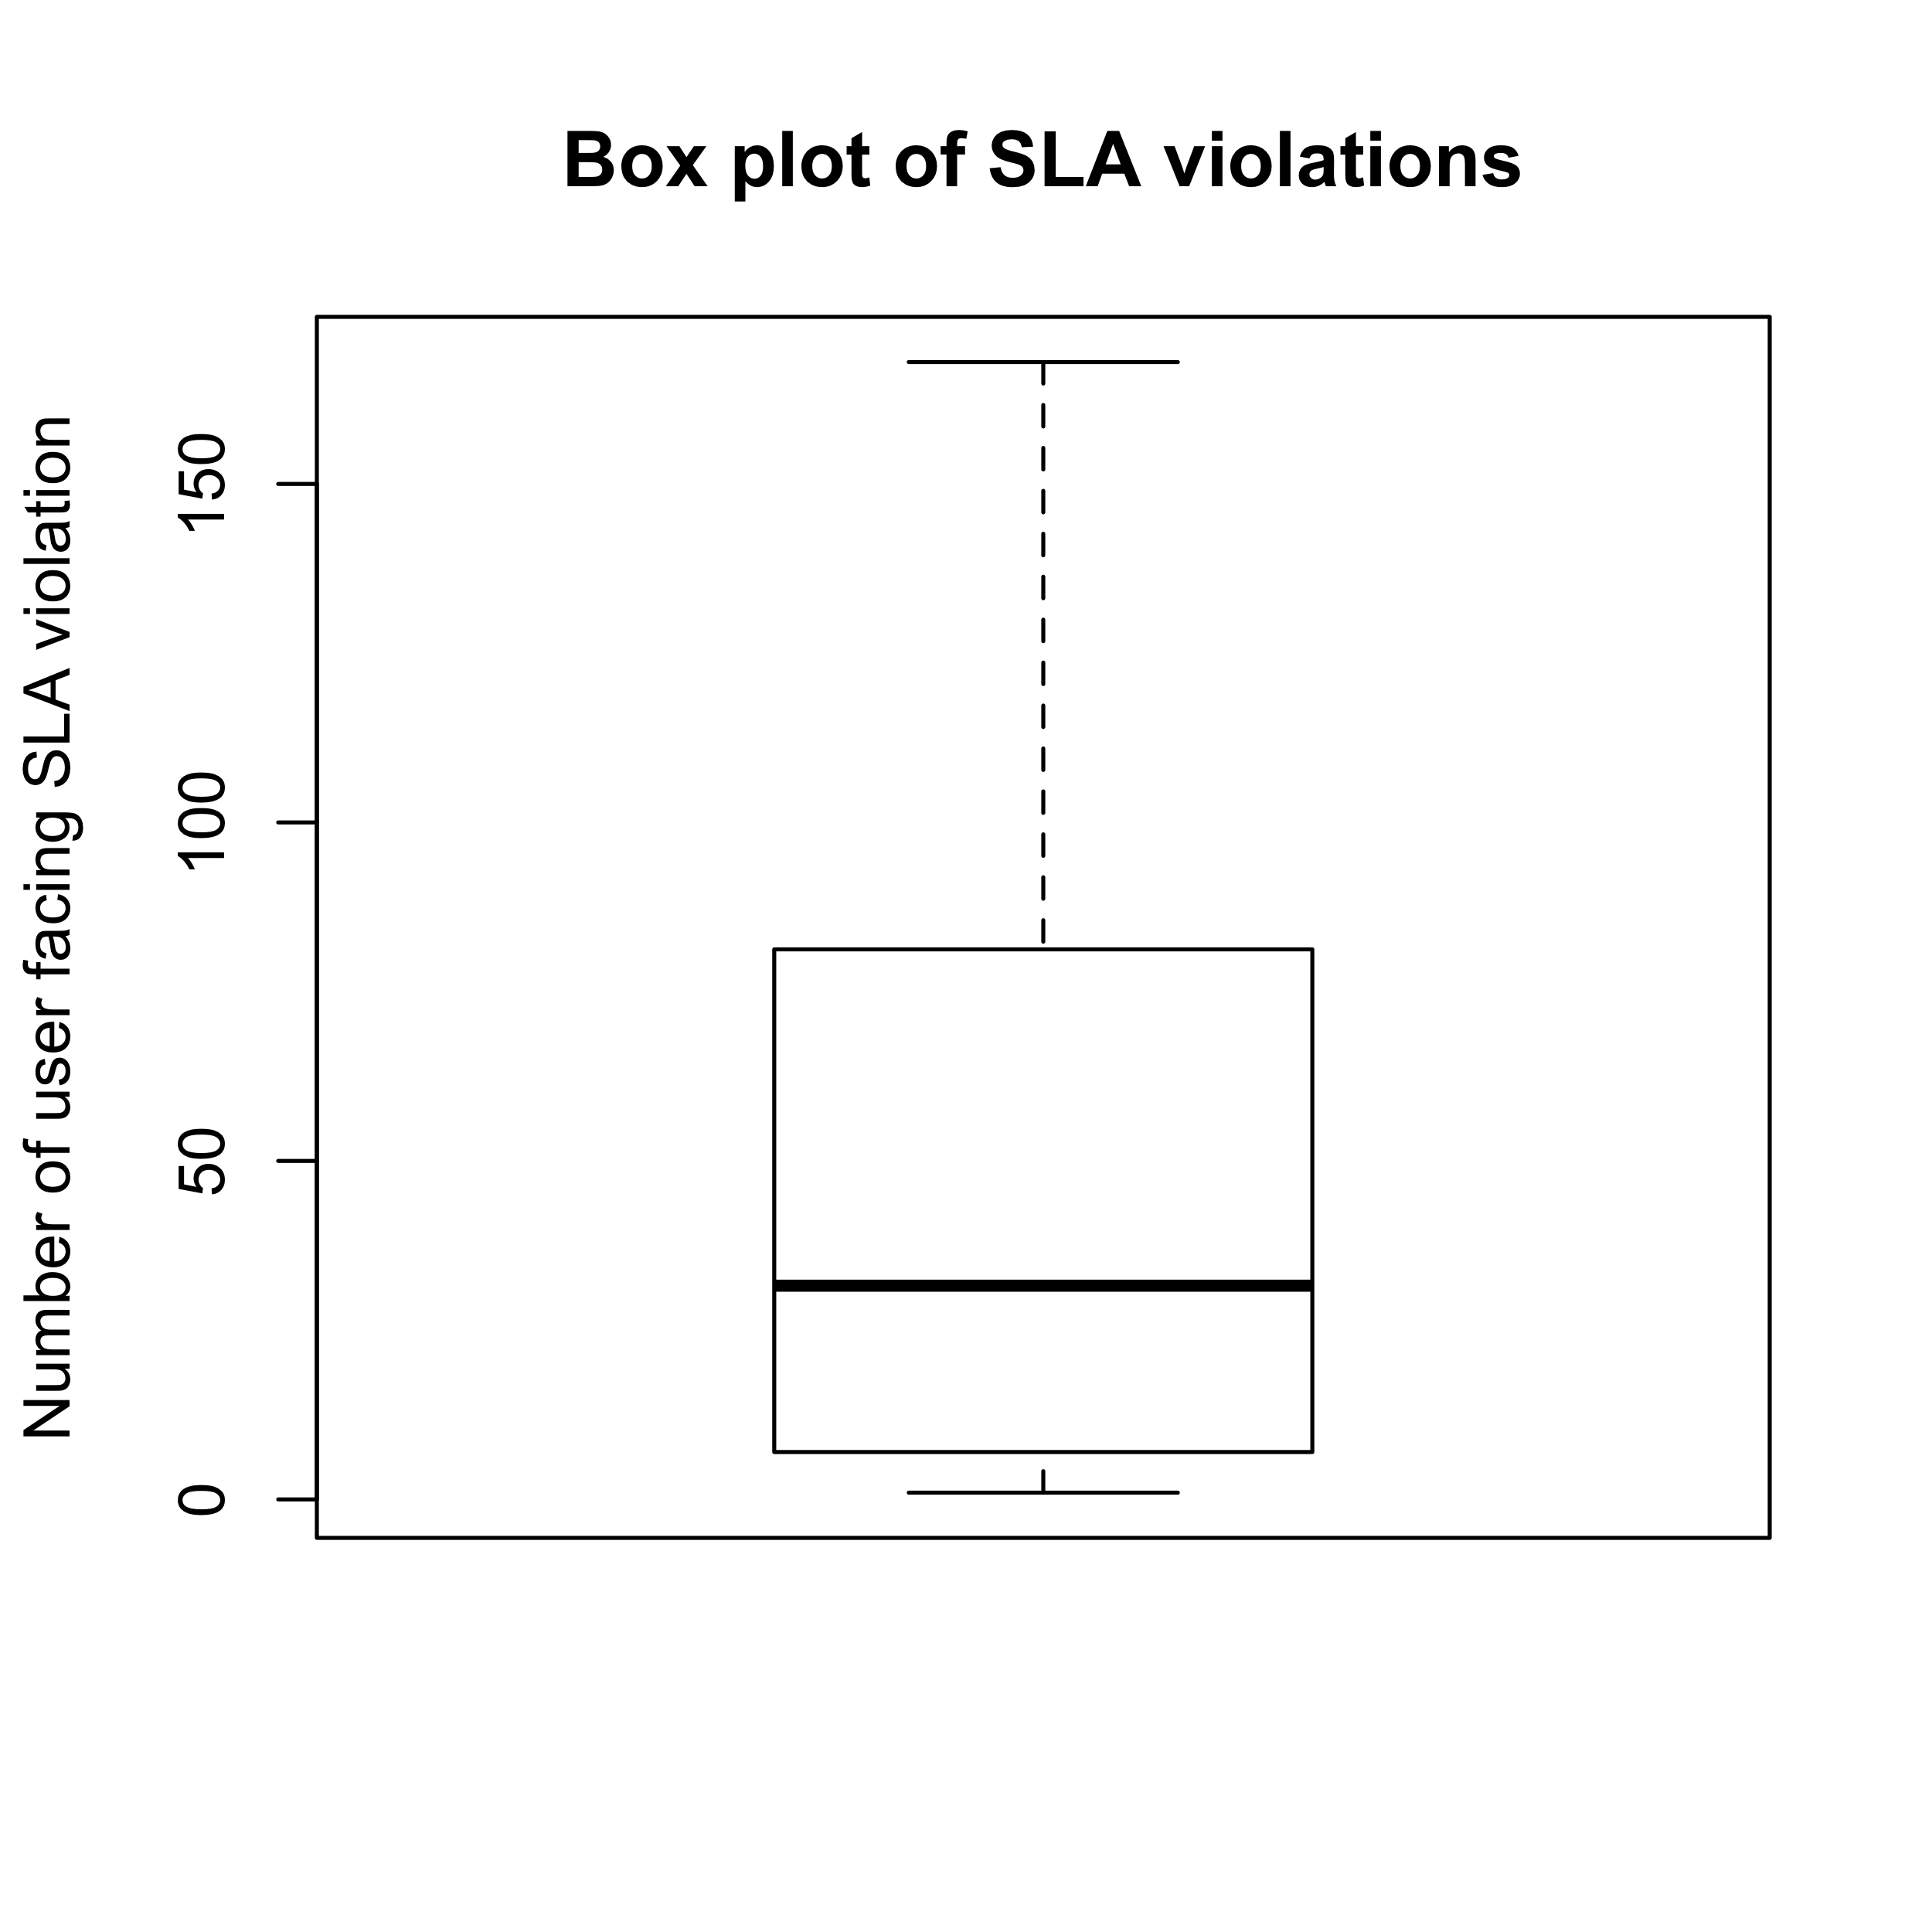
\includegraphics[scale=0.1]{boxplotslaviolation.png}
    \caption{Boxplot of SLA violation}
    \label{figure:boxplotslaviolation}
  \end{center}
\end{figure}
\subsection{Cost Evaluation}
\label{sub:Cost Evaluation}
As discussed in section~\ref{subs:ElasticSim Operation}, ElasticSim given an option of determining how many number of reserved instances to purchase to gain cost benefits\footnote{https://blog.cloudability.com/aws-101-reserved-instances/}. As shown Figure~\ref{figure:purchaseoption}, after running ElasticSim on test workload it produces various option of varying reserved instances. From the Figure~\ref{figure:purchaseoption}, bar graph is grouped into various options. In each option first bar represents the base line price, which is the cost of reserved instances used when serving peak workload. In the scope of this experiment, the base line was calculated for a peak workload of 1070 users. Based on this peak workload, total of 9 VM's are necessary for the period of simulation which is 41 hours and the cost associated with this is USD \$213.2. Since, ElasticSim varies the number of reserve instances to use for providing various option. The second bar represents cost associated with reserving the instances for that particular option. Total number of instances reserved for each option is presented in purple colored bar. Keeping reserved instances fixed through out the simulation, on-demand instances are used for varied workload. The cost associated with on-demand instances are presented in blue bar. The total cost, presented in cyan color, is the sum of reserved instance cost and on-demand instance costs. This total cost is used to make the right instance purchasing choose. Of all the option, option-3 provides a best option for purchasing since the total cost for 3 reserved instance and 18 on-demand instances will cost USD \$158.8. Using purchase option 3, ElasticSim was configured to use total of 3 reserved instances for the simulation duration of 41 hours and the cost benefits of using this option was the saving of USD \$52.45.
\begin{figure}[h]
  \begin{center}
    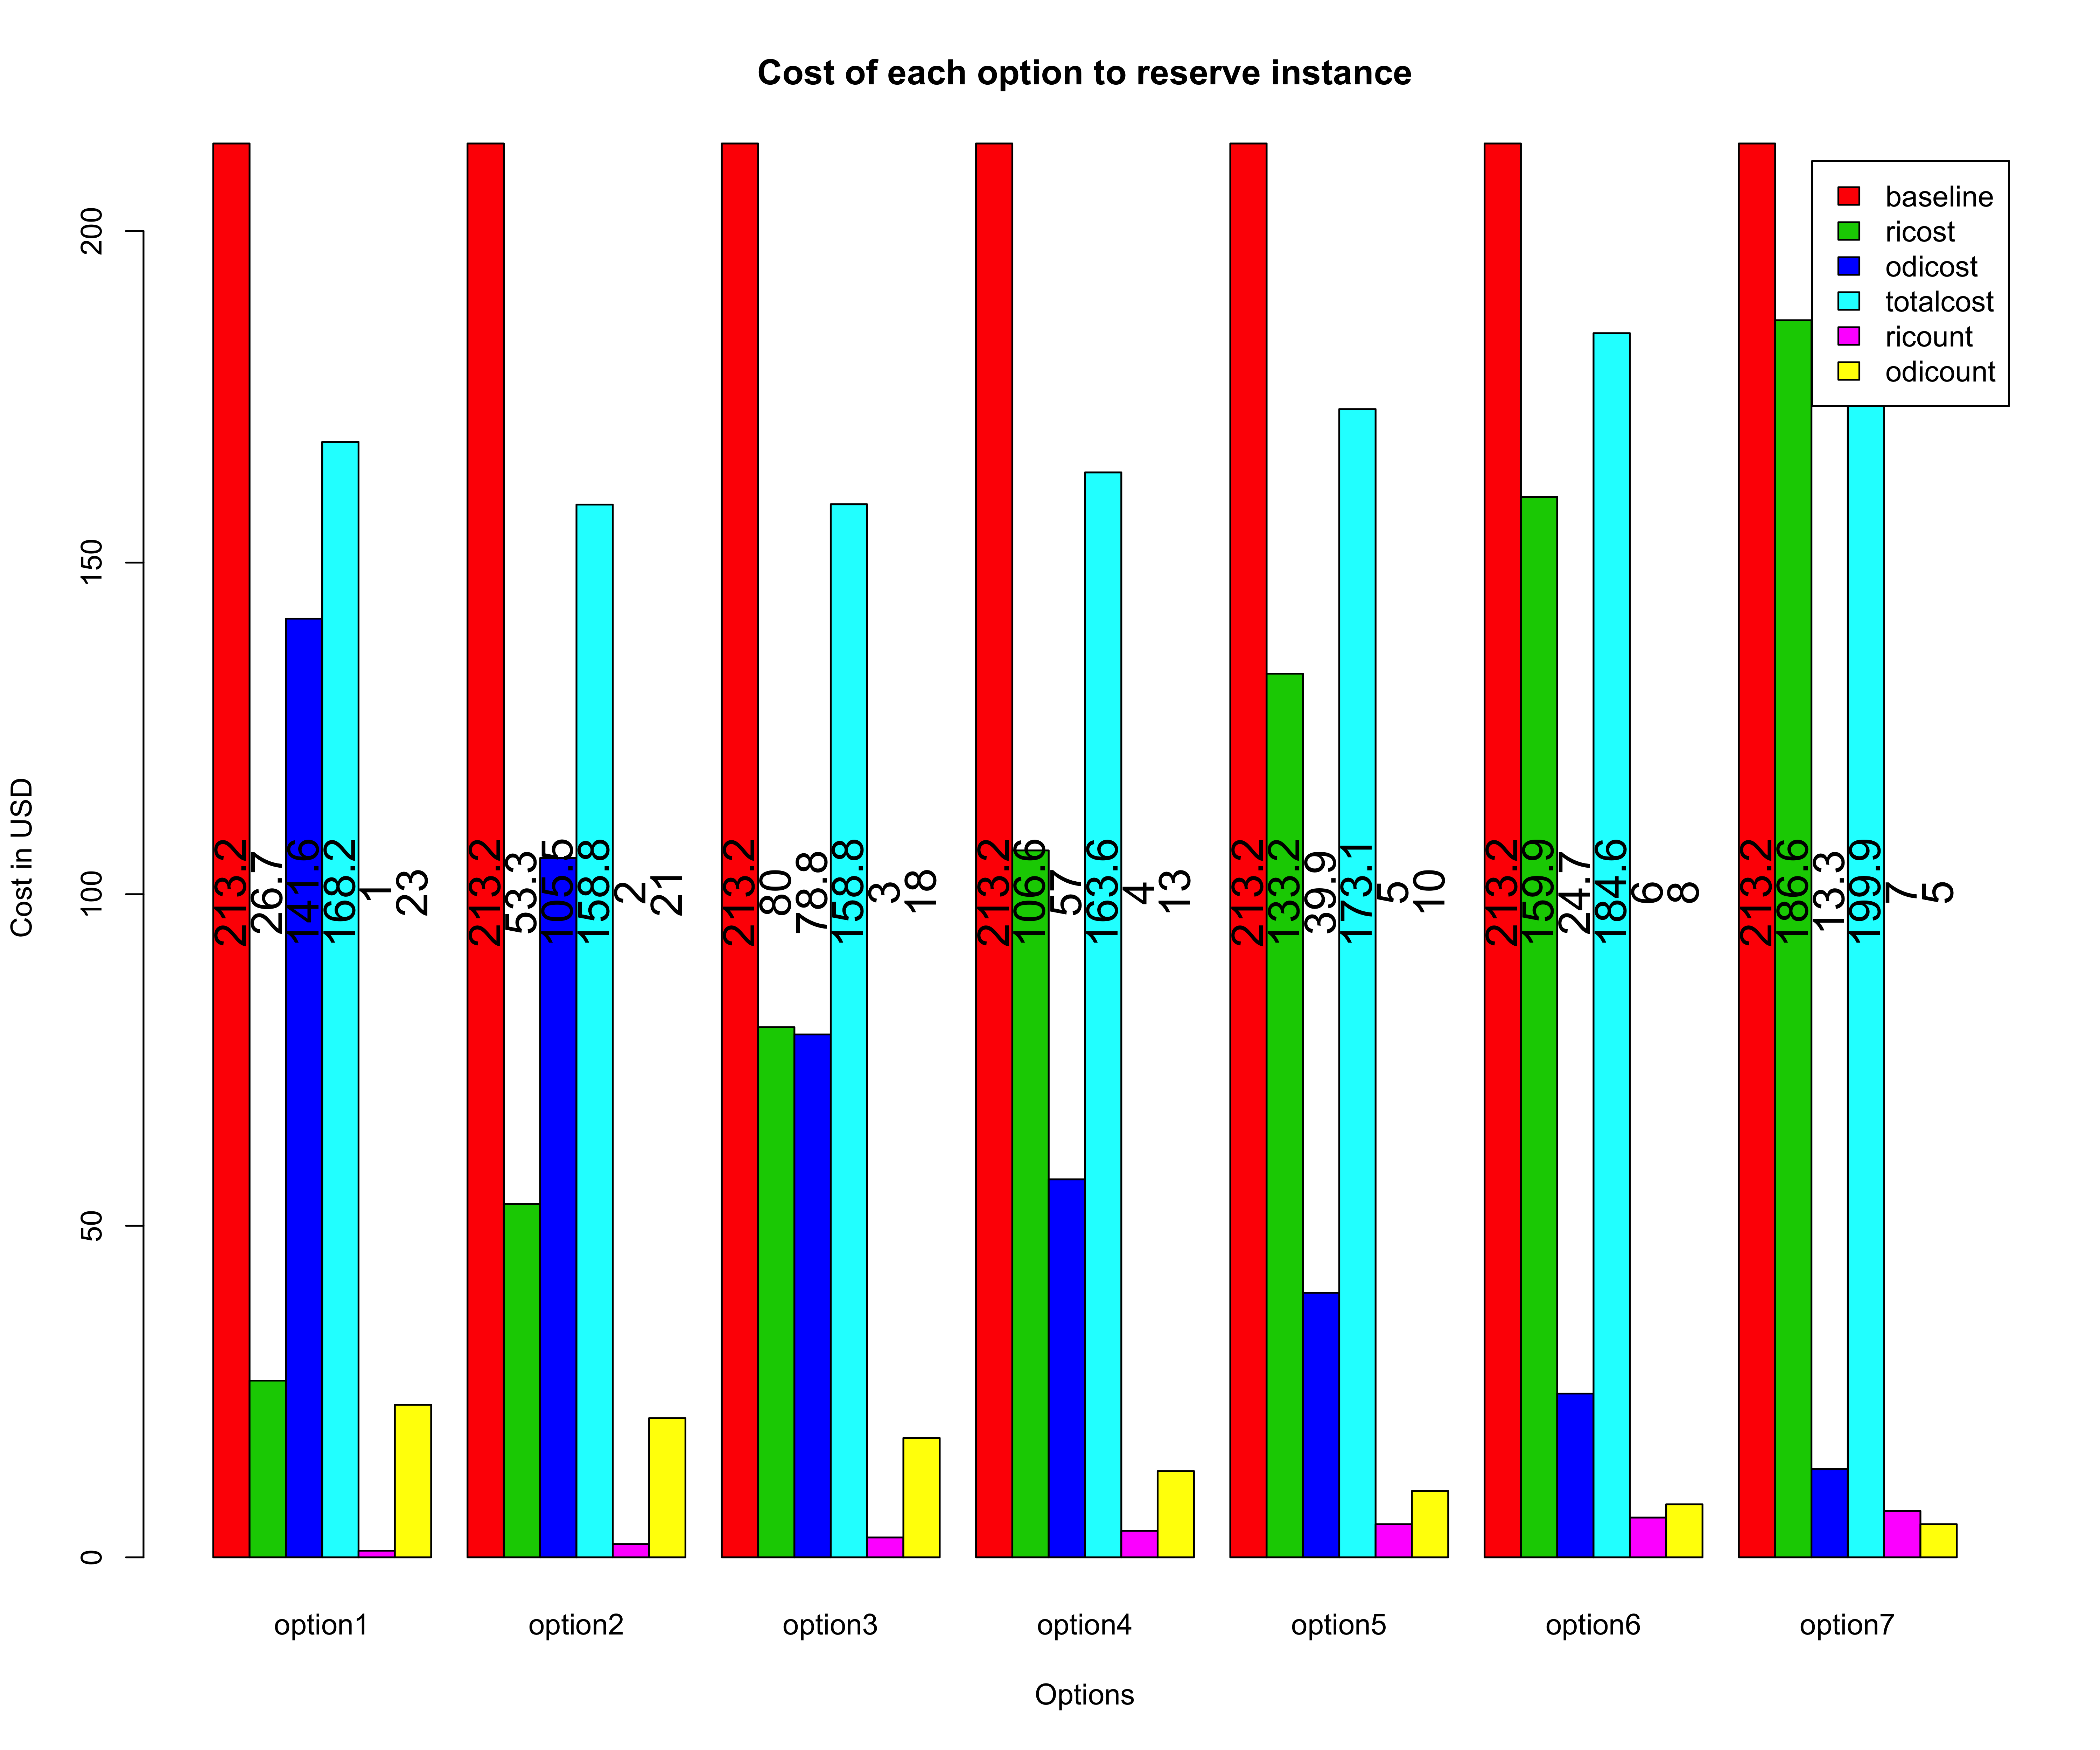
\includegraphics[scale=0.07]{purchaseoption.png}
    \caption{Cost effective instance purchase option}
    \label{figure:purchaseoption}
  \end{center}
\end{figure}

\section{Summary}
\label{sec:Summary}
Section~\ref{section:ElasticSim} provided implementation details of ElasticSim simulator. Implementation details and its internal operations were also presented in this section.
\\
Section~\ref{sec:implementationprediction} implementation details of automated ARIMA forecasting model was presented. Along with forecast model, accuracy measure method called MAPE was explained. In section~\ref{sec:AppElastic Algorithm Implementation}, implementation details and features of AppElastic algorithm was introduced with few code snippets. Proposed approach is evaluated in the section~\ref{sec:Evaluation} through various facets like: effectiveness of AppElastic algorithm, accuracy of ARIMA model and cost benefits. It showed that, deploying AppElastic with optimal reserved instances can provide significant cost benefits.
